%% FEUP THESIS STYLE for LaTeX2e
%% how to use feupteses (English version)
%%
%% FEUP, JCL & JCF, 31 July 2012
%%
%% PLEASE send improvements to jlopes at fe.up.pt and to jcf at fe.up.pt
%%

%%========================================
%% Commands: pdflatex tese
%%           bibtex tese
%%           makeindex tese (only if creating an index)
%%           pdflatex tese
%% Alternative:
%%          latexmk -pdf tese.tex
%%========================================

\documentclass[11pt,a4paper,twoside,openright]{report}

%% For iso-8859-1 (latin1), comment next line and uncomment the second line
\usepackage[utf8]{inputenc}
\usepackage{subcaption}
\usepackage{amsmath}
\usepackage{float}
\usepackage{lscape}
\usepackage{textcomp}
\usepackage{listings}
\usepackage{algorithm}
\usepackage{algpseudocode}
\usepackage{pgfgantt}

\usepackage{xcolor}
    %%-- Customizing the Code Presentation -- %%

\definecolor{codegreen}{rgb}{0,0.6,0}
\definecolor{codegray}{rgb}{0.5,0.5,0.5}
\definecolor{codepurple}{rgb}{0.58,0,0.82}
\definecolor{backcolour}{rgb}{0.95,0.95,0.92}
\definecolor{sectioncol}{HTML}{9C0906}
\definecolor{subsectioncol}{HTML}{CC100C}

\lstdefinestyle{mystyle}{
backgroundcolor=\color{backcolour},   
commentstyle=\color{codegreen},
keywordstyle=\color{magenta},
numberstyle=\ttfamily\tiny\color{codegray},
stringstyle=\color{codepurple},
basicstyle=\ttfamily\scriptsize,
breakatwhitespace=false,         
breaklines=true,                 
captionpos=b,                    
keepspaces=true,                 
numbers=left,                    
numbersep=5pt,                  
showspaces=false,                
showstringspaces=false,
showtabs=false,                 
tabsize=2}
\lstset{style=mystyle}
%\usepackage[latin1]{inputenc}

%% English version

%% MIEIC options
%\usepackage[mieic]{feupteses}
%\usepackage[mieic,juri]{feupteses}
%\usepackage[mieic,final]{feupteses}
%\usepackage[mieic,final,onpaper]{feupteses}

%% MIEEC options
\usepackage[mieec, final]{feupteses}
%\usepackage[mieec,juri]{feupteses}
%\usepackage[mieec,final]{feupteses}

%% For other degrees
%\usepackage{feupteses} % you must define the degree bellow

%% Additional options for feupteses.sty: 
%% - onpaper: links are not shown (for paper versions)
%% - backrefs: include back references from bibliography to citation place

%% Uncomment to create an index (at the end of the document)
%\makeindex
\graphicspath{{figures/}}

%%----------------------------------------
%% TIP: if you want to define more macros, use an external file to keep them
%some macro definitions

% format
\newcommand{\class}[1]{{\normalfont\slshape #1\/}}

% entities
\newcommand{\Feup}{Faculdade de Engenharia da Universidade do Porto}

\newcommand{\mc}[1]{\mathcal{#1}}
\newcommand{\mb}[1]{\mathbf{#1}}

%%----------------------------------------

%%========================================
%% Start of document
%%========================================
\begin{document}

%%----------------------------------------
%% Information about the work
%%----------------------------------------
\title{Dissertation Preparation}
\author{José Pedro Castro Fonseca}

%% Comment next line if not necessary for degree
\degree{Integrated Masters in Electrical and Computer Engineering}

%% Uncomment next line for date of submission
%\thesisdate{July 31, 2008}

%% Comment next line copyright text if not used
\copyrightnotice{José Fonseca, 2016}

\supervisor{Supervisor}{João Canas Ferreira}
\supervisor{Second Supervisor}{Ivo Timóteo}

%% Uncomment next line if necessary
%\supervisor{Second Supervisor}{Name of the Supervisor}

%% Uncomment committee stuff in the final version if used
%\committeetext{Approved by \ldots:}
%\committeemember{President}{Name of the President}
%\committeemember{Referee}{Name of the Referee}
%\committeemember{Referee}{Name of the Referee}
%\signature

%% Specify cover logo (in folder ``figures'')
\logo{uporto-feup.pdf}

%% Uncomment next line for additional text below the author's name (front page)
%\additionalfronttext{Preparação da Dissertação}

%%----------------------------------------
%% Preliminary materials
%%----------------------------------------

% remove unnecessary \include{} commands
\begin{Prolog}
  \pdfbookmark[0]{Table of Contents}{contents}
  \tableofcontents
  \pdfbookmark[0]{List of Figures}{figures}
  \listoffigures
  \chapter*{Abbreviations and Symbols}
%\addcontentsline{toc}{chapter}{Abbreviations}
\chaptermark{Abbreviations and Symbols}

\begin{flushleft}
\begin{tabular}{l p{0.8\linewidth}}
ANN      & Artificial Neural Networks\\
BPTT     & Backpropagation Through Time\\
CNN      & Convolutional Neural Network\\
CPU      & Central Processing Unit\\
FPGA     & Field-Programmable Gate Array\\
LSTM     & Long Short-Term Memory\\
RNN      & Recursive Neural Networks\\
SPSA     & Simultaneous Perturbation Stochastic Approximation\\
\end{tabular}
\end{flushleft}

  % the list of abbreviations used
\end{Prolog}

%%----------------------------------------
%% Body
%%----------------------------------------
\StartBody

%% TIP: use a separate file for each chapter
\chapter{Introduction}\label{chap:intro}
Brief overview of the report:

In Chapter~\ref{chap:intro}, I will present a conceptual background to the problem at hand, exposing the background that surrounds it~\ref{sec:intro_back}, the motivation for the desired solution~\ref{sec:intro_mot}, its objectives~\ref{sec:intro_obj} and, lastly, the people that will help me achieve them~\ref{sec:intro_people}.

In Chapter~\ref{chap:theorBack}, the theoretical foundations will be layed out. Section~\ref{sec:tb_basicCon} presents the basic concepts of Machine Learning, and in the following sections, the theoretical details of ANNs, RNNs and LSTMs. Section~\ref{sec:training_lstm} provides a quick explanation of the training algorithm that will be used in the final solution, which will be outlined in Section~\ref{sec:propSol}.

In Chapter~\ref{chap:workPlan}, the work plan for the Dissertation work is detailed as \emph{tasks} in Section~\ref{sec:wp_tasks_td}, and their temporal arrangement is pictured in a Gantt chart in Section~\ref{sec:wp_tasks_gantt}. Furthermore, the description of the Hardware and Software resources that I will be utilizing during the course of my work is done in Section~\ref{sec:wp_sh}

In Chapter~\ref{chap:stateArt}, the state of the art of LSTMs, their applications~\ref{sec:sa_apps}, their hardware implementations~\ref{sec:sa_hardware} and the current work regarding the chosen training algorithm~\ref{sec:sa_training} are presented.

Finally, in Chapter~\ref{chap:earlyWork} I will present some of the work that I have already concluded.

\section{Background}\label{sec:intro_back}
Artificial Neural Networks are one of the most popular models in the field of Machine Learning. As the name suggests, their operation is inspired by the operation of the building blocks of our brain, the \textbf{neurons}. In spite of its high performance, one of their shortcomings is the fact that they cannot retain temporal dependences among incoming data samples, thus not being suitable to process time-series data, such as audio, video or other kinds of time-varying data streams, where current inputs have a high temporal dependence with previous and future inputs. 

To address this issue, several algorithms have been used, such as Hidden Markov Models (HMM) or Recurrent Neural Networks (RNN), but both of these methods fail to recall temporal dependences that extend over an large period of time, for the reasons that we will understand in Sections~\ref{sec:theorBack_rnn} and~\ref{sec:theorBack_lstm}.Thus, in 1997 Hochreiter et al. proposed a novel RNN structure~\cite{Hoch97}, the Long Short-Term Network (LSTM), where a memory cell was introduced, and the input/output/read/write access is controlled by individual gates that are activated both by the incoming data samples, but also by the outputs from the previous time-step (it is an RNN after all). They are one of the state of the art methods in Deep Learning nowadays, as we can attest in Section~\ref{sec:sa_apps}.

\section{Motivation}\label{sec:intro_mot}
Hitherto, and to the best of my knowledge, all of the published applications that use LSTM are software based, but the parallel nature of the structure hollers for a dedicated hardware realization that can dramatically increase its performance, something that  has only recently been done once~\cite{Chang15} (see Section~\ref{sec:sa_hardware} for further details), and although it improves the processing time when compared to a naïve software solution, it still lacks the ability to perform on-chip learning, and the learning process is performed offline, in a normal CPU, when it also could be sped up by a dedicated hardware structure.

All these techniques are generally implemented in mainstream processors, making use of general high-level or low-level languages, where all the real parallelism is limited to the number of simultaneous threads that we can run on each physical core, which up to now generally have between 2-8 cores (mobile devices and general use personal computers), 

In order to parallelize the computations to the fullest extent, a solution is to port it both to a Graphics Processing Unit (GPU) or even a Field-Programmable Gate Array (FPGA), but the porting process is not entierely automatic and to have the least performance drop possible, it has to be explicitly programmed in CUDA/OpenCL for GPUs, and a Hardware Description Language for FPGAs, with an increasing level of complexity and low-level details. Therefore, it is necessary to provide frameworks that can allow an FPGA to quickly reconfigure itself to run these kind of networks on demand, for a particular task that requires them, achieving a lower computation time, and unburdening the CPU from running it, thus saving performance for running other tasks related with the Operating System, for instance. Furthermore, when processing an incoming stream of highly dimensional data, or with high throughput, a CPU solution might not be scalable, and could benefit greatly from a dedicated hardware implementation.

\section{Objectives}\label{sec:intro_obj}
Taking into account the considerations done in~\ref{sec:intro_mot}, I propose to develop a hardware implementation of an LSTM Network, \emph{with on-chip learning}, improving the performance, capability and flexibility of the existing solution of~\cite{Chang15}. Moreover, I also propose to benchmark this solution and try to compare it with the software performance results of~\cite{Tavear13} and, as a secondary objective, try to use my developed structure to replicate some of the applications portrayed in~\ref{sec:sa_apps}. Lastly, I will work to make this structure reconfigurable on the go, and trying to minimize the reconfiguration time.

\section{People Involved}\label{sec:intro_people}
Besides me, the candidate to the Master's Degree, there are two more people involved, namely

\begin{itemize}
    \item \textbf{Supervisor} -- The \href{https://sigarra.up.pt/feup/pt/func\_geral.formview?p\_codigo=210963}{Professor João Canas Ferreira}, auxiliary professor at the Faculty of Engineering of the University of Porto.
    \item \textbf{Second Supervisor} -- \href{http://www.cl.cam.ac.uk/~ijpdmt2/}{Ivo Timóteo}, MSc, a Computer Science PhD candidate at Cambridge University, UK, in the field of Artificial Inteligence.
\end{itemize}


\chapter{Theoretical Background}\label{chap:theorBack}


\section{Basic Concepts of Machine Learning}
Machine Learning is a field of Computer Science that studies the development of mathematical techniques that allow software to learn autonomously, without an explicit description of each rule of operation. Its goal is to extract latent features from the data that allow an immediate classification of each input data into a particular class -- the catch is that there is no previous rule formulation, but instead we have an adaptive model that adjusts is parameters accordingly with the input data it receives, improving the estimates it yields as it receives new input samples. 

Let us consider a practical example. For instance, suppose we want to build a program that given an input audio waveform representation of a spoken word, it matches it into a particular word of a dictionary. We could, of course, devise a set of rules and exceptions for each word analysing some of its features (perhaps the Fourier representation of each one, and, from it, manually finding the appropriate rules for each), but apart from it being a very complex task, it wouldn't be a scalable solution, given the enormous number of words in each language. The approach taken by Machine Learning is diametrically different, and instead of manually processing each waveform, we build a large dataset, of size $N$, containing the waveforms of several words $\left[ \mb{x}_1 \; \mb{x}_2 \;\mb{x}_2 \; \dots \mb{x}_N \right]$ -- we call this dataset the \textbf{training dataset} -- and we feed it to our model. Each of the $i$-th data point was previously labelled, and in fact we feed each training data point $\mb{x}_i$ \emph{along} with its corresponding label $t_i$, so that the model can adapt its parameters accordingly to the \emph{target value} it is supposed to classify. This set of labels $\mb{t} = \left[ t_1 \; t_2 \; t_3 \; \dots \; t_N \right]$ is called the \textbf{target vector}. 

We are, then, left with the following question: how can the model quantitatively evaluate the quality of its current set of parameters? That could be achieved in a number of ways, but the most usual is using a \textbf{Cost Function} that, as the name suggests, measures the cost of each wrong classification of the model. The model then evolves in a way that minimizes the cost function. A usual choice for the cost function is the \textbf{sum of squares error}. Mathematically, if $y_{\theta}^i = y_{\theta}(x_i)$ is the prediction for the input data point $x_i$ with label $t_i$, given the current set of parameters $\theta$, the cost function using this metric is given by

\begin{equation}\label{eq:costfunctionFund}
	J(\theta) = \frac{1}{2} \sum_{i=1}^N \left( y_{\theta}^i - t_i \right)^2.
\end{equation}

Sometimes, instead of applying the raw data to the model, we can apply some sort of \emph{preprocessing} to the data to extract the relevant features from it. For instance, instead of just feeding a raw image, we can perform several operations like edge detection or low-pass filtering, and apply them in parallel. In cases of highly dimensional data (i.e. each data vector has a very high number of features), we can apply techniques like \textbf{Principal Component Analysis} to reduce the feature space to a smaller dimension one, where the previous features were combined into two or three new features that pose themselves as the most relevant.

The problems described above are, in fact, a subset of the problems that Machine Learning tries to address. These problems are called \textbf{classification problems}, because for each input data point, our model tries to fit it into the most appropriate class. But we can also address \textbf{regression problems} where the output is not limited to a discrete set of values but rather a continuous interval. On the other hand, the Neural Network that this work will implement addresses a special kind of classification problem, where the classification decision is influenced not only by the current input sample, but also by a given \emph{window of samples} that trail the current sample.

In summary, the most typical setting for a Machine Learning problem is having a large \textit{input dataset} which we use to \textit{train} our model (i.e. allowing him to dynamically adapt its set of parameters $\theta$), in order to produce an output label $y_i$ for each of them that minimizes a quality metric, the \textit{Cost Funcion}, which can be chosen to the sum of squared differences, the log-loss, or any other appropriate  mathematical relationship  between the estimate $y_i$ and the correct label $t_i$. 

Now that the basic Machine Learning concepts have been presented, I will discuss, henceforth, one of the most important algorithms that address the supervised classification problems, the \emph{Artificial Neural Networks} that will be discussed in Section~\ref{sec:theorBack_ann} as somewhat of a contextual introduction to the main theme of the thesis, which will be Recurrent Neural Networks (Section~\ref{sec:theorBack_rnn}), namely the \textbf{Long Short-Term Memory Networks} (Section~\ref{sec:theorBack_lstm}), both of which are improvements over the initial formulation of the ANNs. These two last networks branch even further from these set of problems, and are usually employed in \textit{Deep Learning} tasks, where we try to extract even higher level information from data at the expense of increased model complexity. 

\section{Artificial Neural Networks}\label{sec:theorBack_ann}

Artificial Neural Networks (ANN) are mathematical structures that, as the name suggests, try to mimic the Human Brain. ANN's building blocks, like their biological counterpart, model the high-level behaviour of biological neurons, in the sense that they neglect unnecessary biological aspects (such as modeling all the voltages across the neuron and all its electromagnetic interactions), and only retain its fundamental underlying mathematical function, which is a weighted linear combination of its inputs subject to a \emph{activation function}, i.e. a function that outputs a decision value depending on its inputs.  Mathematically, we have

\begin{equation}
	y = f(\mb{w}^T \mb{x} + b_0)
\end{equation}
where $\mb{w} = \left[ w_1 \; w_2 \;  w_3 \;  \dots \; w_n \right]$ is the input weight vector, $\mb{x} = \left[ x_1 \; x_2 \; x_3 \; \dots \; x_n \right]$ the input vector, $b_0$ is the bias factor and $f(\cdot)$ is the chosen activation function. Furthermore, we call the scalar quantity $a = \mb{w}^T \mb{x} + b_0$ the \textbf{activation}, since its value determines how the activation function will behave. Figure~\ref{fig:modelNeuron} exemplifies the roles of these variables within our neuron model, and compares each part of it with the biological counterpart.

\begin{figure}[!H]
	\begin{subfigure}{0.5\linewidth}
		\centering
		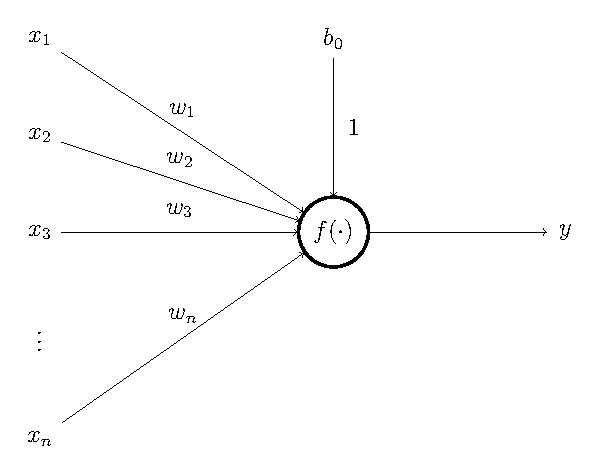
\includegraphics[width=0.9\linewidth]{figures/neuron.eps}
		\caption{Neural Network Node}
		\label{fig:modelNeuron_a}
	\end{subfigure}
	\begin{subfigure}{0.5\linewidth}
		\centering
		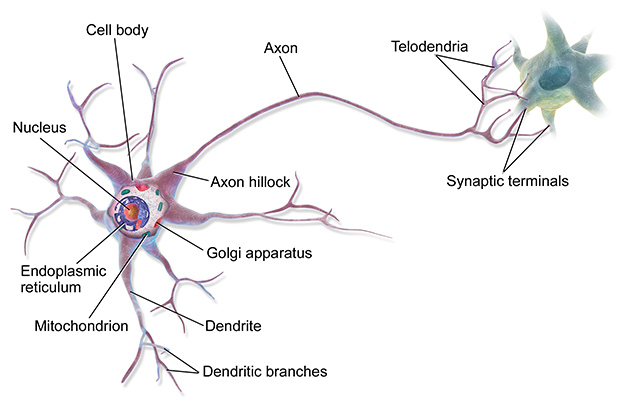
\includegraphics[width=0.9\linewidth]{figures/multipolarNeuron.png}
		\caption{Biological Neuron Diagram}
		\label{fig:modelNeuron_b}
	\end{subfigure}
		
	\caption{In Figure~\ref{fig:modelNeuron_a}. each input feature $x_i$ is weighted by its corresponding weight $w_i$. During the training procedure, these weights are adjusted so that the output $y$ approaches the target value. In Figure~\ref{fig:modelNeuron_b}, we see the diagram of an actual multi polar neuron. The dendrites, where the stimuli are received, plays a role similar to that of the input nodes. The axon transmits the signal to the synaptic terminals, that are similar to the $y$ output}
	\label{fig:modelNeuron}
\end{figure}


As far as the activation function is concerned, we can have several types. An immediate choice would be the \textbf{Binary Step Function} that  outputs -1 if the activation is \textbf{below} a given threshold and 1 otherwise. There can also be \textbf{real valued activation functions}, whose output is not binary, but rather that of a continuously differentiable function, such as the logistic sigmoid $\sigma(a) = \frac{1}{1 + \mathrm{e}^{-a}}$ or the hyperbolic tangent $\tanh(a)$. This aspect will prove useful for the usual training methods, that involve the computation of derivatives. In Figure~\ref{fig:activFunc} these activation functions are plotted.

\begin{figure}[H]
	\centering
	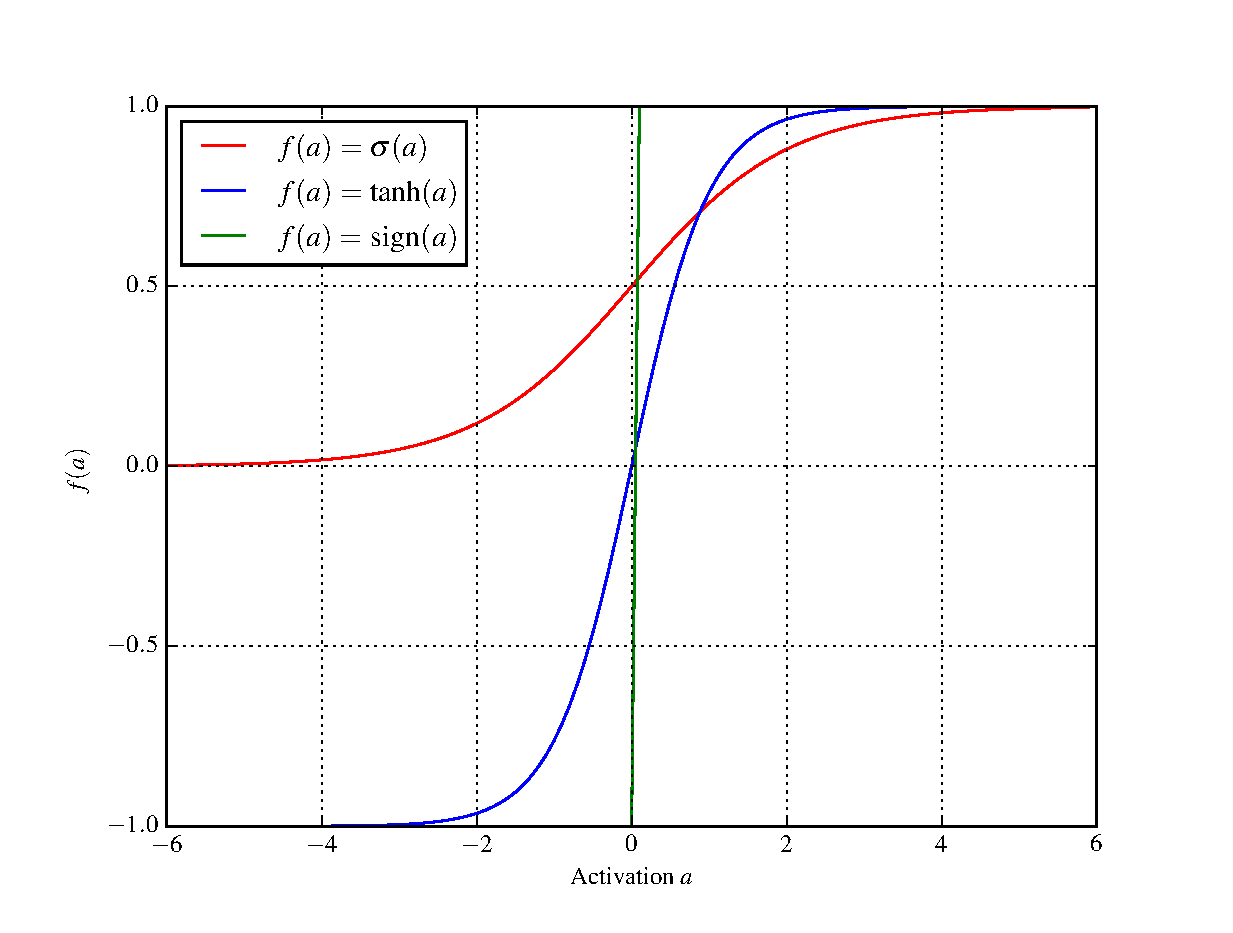
\includegraphics[width=0.9\linewidth]{figures/activFunc.eps}
	\caption{Three different activation functions. As you can see, the hyperbolic tangent has the same extreme value as the sign step function, but has a smooth transition between them, which can be interpreted as a \emph{soft decision} in the more ambiguous middle region, reflecting the degree of uncertainty on the decision. On the other hand, the sigmoid function goes from zero to one, and is also smooth like the hyperbolic tangent}.
	\label{fig:activFunc}
\end{figure}


A neuron by itself can be thought of as a simple linear regression, where we optimize the weight of each feature according to a target value, or function. While important in some applications, the main interest in ANN is to evaluate increasingly more complex models, and not a simple linear regression. This is achieved by \emph{chaining} nodes to one another, connecting the output of a given node to one of the inputs of another. We call \emph{layers} to a group of these nodes that occupy the same hierarchical position. There can be any number of layers, with any number of nodes, but most implementations generally have 3 layers: the \emph{initial} layer, the \emph{hidden} layer (in the middle) and the \emph{output} layer. Figure~\ref{fig:neuralnet} suggests a possible structure for a 3 layer ANN. 


\begin{figure}[H]
	\centering
	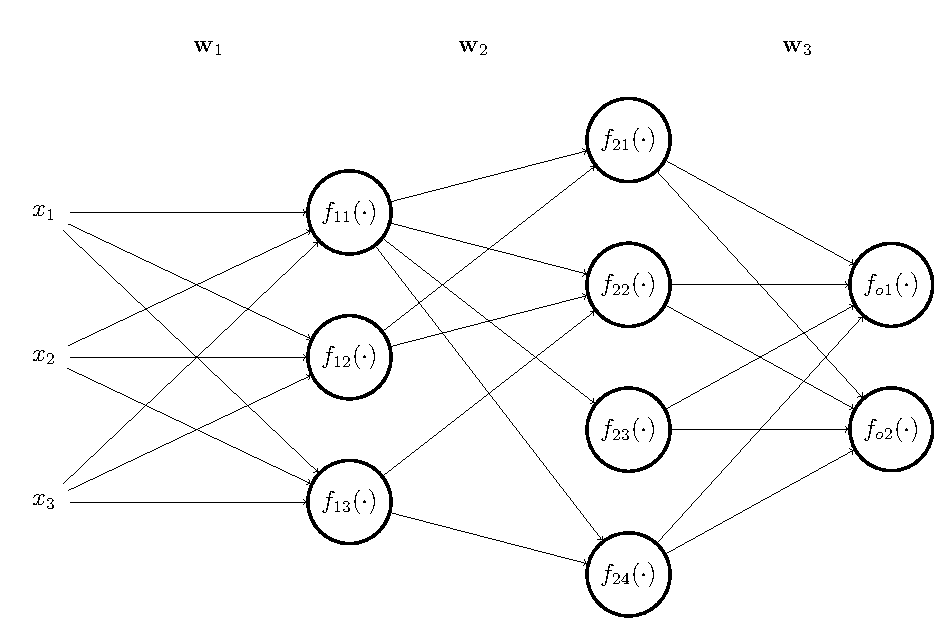
\includegraphics[width=0.9\linewidth]{figures/ann.eps}
	\caption{A three layer ANN. We have omitted some of the connections in the hidden layer, for simplification purposes. $\mb{w}_1$ represents the weight matrix of the input layer, $\mb{w}_2$ the weight matrix of the connections between the input layer and the hidden layer, and $\mb{w}_3$ the weight connections between the hidden and the output layer. $f_{ij}(\dots)$ is the activation function of the $j$-th neuron of the $i$-th layer. Since they can be different, I chose different indexes to each.}
	\label{fig:neuralnet}
\end{figure}

Regarding the training of ANNs, is is performed through a two-step process: first, a \textbf{feed-forward} step where the input is applied, and the activations are evaluated in succession up to the output neurons; then, the perform the \textbf{backpropagation} step, where we calculate the errors in each of the nodes, but now from the output to the input: the weights are updated and optimized using an iterative  method called \textit{Gradient Descent}, where if $\tau$ is the current time step, the next update on the weight matrix $\mb{w}^{(\tau+1)}$ is given by

\begin{equation}\label{eq:gradDesc}
	\mb{w}^{(\tau+1)} = \mb{w}^{(\tau)} - \eta \nabla E(\mb{w}^{(\tau)})
\end{equation}
where $E(\cdot)$ is the error function. As we can see, the weight matrix is moved in the direction that minimizes the error function the most, and $\eta$ controls how fast this is achieved, being the reason why it is called the \textbf{learning rate}.

The computation of gradient of the error function comprises the evaluation of its derivatives with respect to each weight of all network connections, $w_{ij}$. They are

\begin{equation}\label{eq:partialE}
	\frac{\partial E}{\partial w_{ji}} = \delta_j f(a_i)
\end{equation}
where $f(\cdot)$ is the activation function of the neuron and

\begin{equation}\label{eq:deltaj}
	\delta_j = f'(a_j) \sum_k w_{kj} \delta_k .
\end{equation}
The interpretation of these equations is simple. If $w_{ji}$ is the weight of the connection between the neuron $j$ we are considering and a neuron $i$ in a previous layer, then the sum over $k$ relates to all the neurons in the \emph{next} layer to which $j$ connects: this way, since the update on $w_{ji}$, according to~\ref{eq:gradDesc}, is given by

\begin{equation}\label{eq:update}
	w_{ji}^{(\tau+1)} = w_{ji}^{(\tau)} - \eta \frac{\partial E}{\partial w_{ji}}
\end{equation}
we see that, from~\ref{eq:partialE}  it simply is the product of the error of the current neuron, $\delta_j$, with the output of the previous neuron $f(a_i)$. In turn, from~\ref{eq:deltaj}, we see the recurrence relationship between it and the weighted sum of all posterior neurons that connect to it. Hence, the name backpropagation is now clear: we are, in fact, propagating the errors backwards into the neuron of interest, weighted by the corresponding weight, but now \emph{backwards} instead of forward, as before. For the output units, the $\delta_j$ is simply the difference between the produced output and the corresponding label for that sample. This two-step process is performed for every data point in out dataset. %%Place where I can include an algorithmic overview?
For a complete proof of the above formulas, see~\cite[chap. 5.3.1]{Bishop2006}.

\section{Recurrent Neural Networks}\label{sec:theorBack_rnn}
A Recurrent Neural Network (RNN) is, essentially, a regular ANN where some neurons (especially in the hidden layer) have \emph{feedback connections} to themselves, i.e. their outputs are fed as inputs. The relevance of this different structure is the possibility to retain \emph{sequence} information about the data. Before, each incoming data point only contributed to the training of the network, but no information about the correlation between themselves and the data points that preceded them did not influence the training step. They were regarded as if no temporal relationship existed, and therefore each data point is conditionally independent of any other. This is obviously not necessarily truth, and in fact there are many cases, where the correlation between data points is high for those closely spaced in time, in which it is actually completely false, as in video signals, audio signals, or other kinds of \emph{temporal sequences} of data. Therefore, the feedback connection of the neuron to himself acts as a kind of \emph{memory element} that takes into account in the present decision, the history of decisions previously taken, and hence the previous data. 
Figure~\ref{fig:recneuron} suggests a possible structure for a neuron of a hidden layer in an RNN, and also an alternate representation, where the structure is unfold through time.

%% METE AQUI A FIGURA

The training of an RNN is usually performed using a variation of Backpropagation, called \textbf{Backpropagation Through Time} (BPTT), that as the name implies, performs the same backpropagation procedure discussed for the ANNs, but now taking into account the unfolding of the network through a fixed training epoch $T$ like Figure~\ref{fig:recneuron}. Due to this very fact, this training procedure is memory and performance consuming, and so it will not be used in my final work, but instead a novel approach, the \textbf{Simulatneous Perturbation Stochastic Approximation}. 

Even though RNNs outperform static ANNs in sequence recognition problems~\cite{Bengio1991}, they fail to retain long-term dependencies. Of course that the weight training process is itself a form of memory, but the problem is that the weight update is much slower than the activations~\cite{Yoshua01}, and therefore this memory only retains short-term dependencies. This is because of the so-called \textbf{Vanishing Gradients Problem}~\cite{Yoshua94,Yoshua01}, where the error decays exponentially through time, and the impact of previous incoming data points on the training of the weights, and thus the current decision, quickly decreases. 


\section{Long Short-Term Memory Networks}\label{sec:theorBack_lstm}
To overcome the issue of failing to remember long-term dependencies, Hochreiter and Schmidhüber proposed, in 1997, a novel approach to the RNNs called the \textit{Long-Short Term Network}~\cite{Hoch97}. This section explains the main idea of this approach~\ref{sec:struct_lstm}, and also how it is trained\ref{sec:training_lstm}, serving as a support basis for the work of this thesis.
Although originally formulated in 1997, its formulation has been incrementally updated in~\cite{Gers00} and~\cite{Gers2000}, and the most current version is the one in~\cite{Graves05}. One of the inital proposers of LSTM, Prof. Jürgen Schmidhüber, did a survey on the most common variations of the structure~\cite{Greff15} last year, and this will the basis of this short theoretical presenation, as well as the work that will be developed in this thesis. 

\subsection{Structure, Operation and Equations}\label{sec:struct_lstm}
A single LSTM neuron is presented in Figure~\ref{fig:lstmneuron}. As we can see from the picture, we still have the recurrent connections from the regular RNNs, but now there are multiple entry points that control the flow of information through the network. Although ommited from the  picture, all the gates are biased, as is suggested in Equations~\ref{eq:equationsLstm}. The main components, their role and relevance, are explained as follows

\begin{itemize}

    \item \textbf{Input Gate} -- this is the input gate, where the importance of each feature of the input vector at time $t$, $\mb{x}^t$, and the output vector at the previous time step $\mb{y}^{t-1}$ is weighed in, producing an output $\mb{i}^{t}$.

    \item \textbf{Block Input Gate} -- as the name implies, this gate controls the flow of information from the input gate to the memory cell. It also receives the input vector and the previous output vector as inputs, but it does not have peephole connections and its dynamics are controlled by a different set of weights. The \textbf{activation function of this gate can be any}, but the most common choice is the \textbf{Hyperbolic Tangent}.

    \item \textbf{Forget Gate} -- its role is to control the contents of the Memory Cell, either to set them or reset them, using the \textit{Hadamard Elementwise} matrix multiplication of its output at time $t$, $\mb{c}^{(t)}$, with the contents of the memory unit at the previous time step, $\mb{c}^{(t-1)}$. The activation function of this gate is \textbf{always sigmoid}.

    \item \textbf{Output Block Gate} -- this gate has a role very similar to that of the Block Input Gate, but now it controls the information flow \textit{out} of the LSTM neuron, namely the activated Memory Cell output.

    \item \textbf{Memory Cell} -- the cornerstone of the LSTM neuron. This is the memory element of the neuron, where the previous state is kept, and updated accordingly to the dynamics of the gates that connect to it. Also, this is where the peephole connections come from:  

    \item \textbf{Output Activation} -- the output of the Memory Cell goes through this activation function that, as the gate activation function, can be any, but the \textit{hyperbolic tangent} is the most common choice.

    \item \textbf{Peepholes} -- direct connections \textit{from} the memory cell that allow for gates to `peep' the states of the memory cell. They were added after the initial 1997 formulation, and their absence was proven to have a minimal performance impact~\cite{Greff15}.
\end{itemize}

After this small conceptual definitions, that allow us to grasp some intuition on the operation of a \textit{single} LSTM cell, I can present the overview of a \textit{layer} of LSTM neurons and their formal mathematical formulation, that will be needed both for the high-level model and the HDL description. The operation of each gate of the layer is given by the following set of equations

\begin{align}
    \mb{z}^{(t)} & = g(\mb{W}_z \mb{x}^{(t)} + \mb{R}_z \mb{y}^{(t-1)} + \mb{b}_z) \\
    \mb{i}^{(t)} & = \sigma(\mb{W}_i \mb{x}^{(t)} + \mb{R}_i \mb{y}^{(t-1)} + \mb{p}_i \odot \mb{c}^{(t-1)} + \mb{b}_i) \\
    \mb{f}^{(t)} & = \sigma(\mb{W}_f \mb{x}^{(t)} + \mb{R}_f \mb{y}^{(t-1)} + \mb{p}_f \odot \mb{c}^{(t-1)} + \mb{b}_f) \\
    \mb{c}^{(t)} & = \mb{i}^{(t)} \odot \mb{z}^{(t)} + \mb{f}^{(t)} \odot \mb{c}^{(t-1)} \\
    \mb{o}^{(t)} & = \sigma(\mb{W}_o \mb{x}^{(t)} + \mb{R}_o \mb{y}^{(t-1)} + \mb{p}_o \odot \mb{c}^{(t)} + \mb{b}_o) \\
    \mb{c}^{(t)} & = \mb{o}^{(t)} \odot h(\mb{z}^{(t)}) 
\end{align}
The $i$-th element of the previous vectors in bold corresponds to the value of the gate of the $i$-th neuron of the layer, which is a very convenient and compact representation of the whole layer. Although useful for a high-level description in a programming language, the matrix representation  may not be suitable for a direct HDL port. In that case, all the above equations still hold, but instead of \textit{vectors} of outputs, we will have a single output, and we only use the appropriate value in the weight matrices $\mb{W}_{\cdot}$ and $\mb{R}_{\cdot}$
\begin{figure}
	\centering
	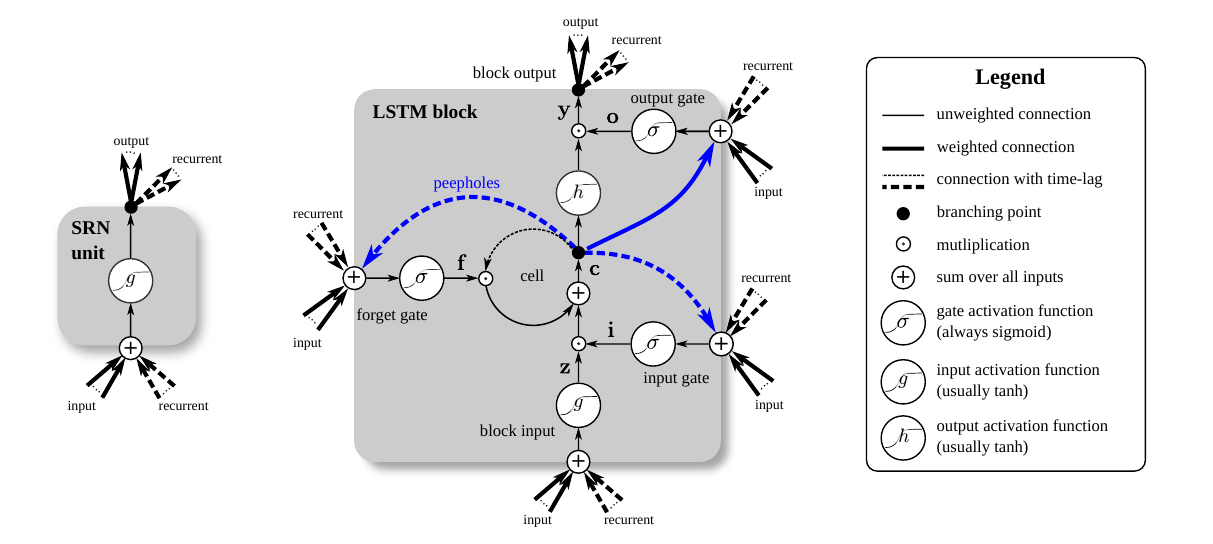
\includegraphics[width=0.9\linewidth]{figures/lstmneuron.png}
    \caption{A complete LSTM neuron, with all the features as described in~\cite{Graves05}}
	\label{fig:lstmneuron}
\end{figure}

\subsection{Training -- SPSA}\label{sec:training_lstm}
Since this work aims to perform on-chip learning, it is important to find a suitable learning scheme. Since I am aiming at an hardware implementation, and although the memory resources of nowadays FPGAs are abundant, one must find an algorithm that uses the less memory as possible (at the smallest performance cost possible), in order to use the additional memory, for instance, to add additional LSTM cells that can improve the performance of our system. 
That being said, we see that the usual training algorithms for LSTM cells -- i.e. Real-Time Recurrent Learning (RTRL), Truncated Backpropagation Through Time (BPTT) or a mixture of both~\cite{Graves05}~\cite{Hoch97}~\cite{Greff15} -- usually involve the storage of the deltas of each layer for every time instant in the training epoch (from $0$ to $T$), which is a highly non-scalable solution both in terms of memory and performance. A most efficient approach to training times series dependant structures like LSTM is the use of \textbf{Simultaneous Perturbation Stochastic Approximation} (SPSA)~\cite{Spall98}. The weight update for the $i$-th weight at the time step $t$ is given by 

\begin{equation}\label{eq:spsa_weightUpdate}
    \Delta w_i^{(t)} = \frac{J(\mb{w}^{(t)} + \beta \mb{s}^{(t)}) - J(\mb{w}^{(t)})}{\beta s_i^{(t)}}
\end{equation}
where $\beta$ is the magnitude of the perturbation to be introduced, $\mb{s}^{(t)}$ is a \textit{sign vector} whose $i$-th element, $s_i^{(t)}$, is either $-1$ or $1$. This way, we see that every weight is \textbf{randomly} incremented either by $-\beta$ or $\beta$, and we only need to keep a duplicate of the weight matrix with the perturbations, and we only need to evaluate the cost function twice per incoming sample. As for the \textit{update rule} is concerned, we have 

\begin{equation}\label{eq:spsa_updateRule}
    w_i^{(t+1)} = w_i^{(t)} - \eta \Delta w_i^{(t)}
\end{equation}
where $\eta$ is the learning rate, and $\Delta w_i^{(t)}$ is the update for the $i$-th weight evaluated in~\ref{eq:spsa_weightUpdate}.
According to the analysis performed in~\cite{Maeda05}, performing a second-order Taylor expansion at $\mb{w} = \mb{w}^{(t)}$, and taking the expected value of the equation, we get that

\begin{equation}\label{eq:spsa_gradProof}
    E(\Delta w_i^{(t)}) = \frac{\partial J(\mb{w}^{(t)})}{\partial w_i^{(t)}}
\end{equation}
that is, the weight update approximates the gradient of the cost function relative to that weight, and so the learning rule is a special form of \textit{Stochastic Gradient Descent}.

One last comment to be made concerning the update rule, is the hipothetical need for \textbf{limits} to the weight values, when the update rule exceeds $|w_{\text{max}}|$ (in that case, we set $w_i^{(t+1)} = \pm w_{\text{max}}$), which sometimes might be needed if the behaviour of the weight update is not appropriate~\cite{Maeda05}.



\chapter{State of the Art}\label{chap:stateArt}

Over the course of this chapter, I am going to present an overview of the most recent developments related to the work of this thesis, both in terms of existing dedicated hardware implementations~\ref{sec:sa_hardware}, the most relevant work in adapting suitable training algorithms to hardware~\ref{sec:sa_training} and also some of the most relevant applications of LSTM~\ref{sec:sa_apps}, which are not FPGA-based, but demonstrate how LSTM is useful by itself, and how well it competes with other Machine Learning algorithms in terms of long time-series dependences in data.

\section{LSTM Applications (non-FPGA related)}\label{sec:sa_apps} 
LSTM Networks are nowadays one of the state of the art algorithms in deep-learning, and their performance is superior to that of other kinds of RNNs and Hidden Markov Models, both of which are generally used to address the same set of problems where LSTM are employed, namely predicting and producing classification decisions from time-series data \textbf{citation needed!}. A very comprehensive description of applications can be found in one of the initial authors webpage dedicated to the subject~\footnote{\href{http://people.idsia.ch/~juergen/rnn.html}{http://people.idsia.ch/~juergen/rnn.html}}. I will now enumerate some of the bleeding edge applications of LSTM.

\begin{itemize}
    \item \textbf{Handwriting Recognition} -- and LSTM-based network~\cite{Bertolami09}, submitted by a team of the Technische Universität München, won the 2009 ICDAR Handwriting Recognition Contest, achieveing a recognition rate of up to 91\%~\cite{ICDAR09}. LSTMs have also proven to surpass HMM based models in terms of optical character recognition in printed text, as~\cite{Breuel13} suggests.

    \item \textbf{Speech Recognition} -- an architecture\cite{Graves13} proposed by Graves et al. in 2013 achieved an astonishing 17.7\% of accuracy on the TIMT Phoneme Recognition Benchmark, which up to the date is a new record. Furthermore, it has also been used for large scale acoustic modelling of speech~\cite{Sak14}.

    \item \textbf{Handwriting Synthesis} -- a comprehensive study by Graves shows, among other sequence generation tasks such as Text Prediction, the use of LSTM to produce synthetic handwriting, that looks incredibly similar to human-produced handwriting~\cite{Graves13_2}.

    \item \textbf{Translation} -- LSTM was used by Sutskever et al. (Google) to perform sequence-to-sequence translation on the WMT'14 dataset, translating English to French with a close to state of the art score~\cite{Sustkever14}.

    \item \textbf{Biomedical Applications} -- this network architecture was used in a protein homology detection scheme~\cite{Hochreiter07} using the SCOP 1.53 benchmark dataset, displaying a staggering performance when compared to other methods. Similarly, a recent article from 2015 by Sønderby et al. suggested the use of standalone LSTM and also Convolutional LSTM to perform subcellular localization of proteins, given solely their protein sequence, with an astounding accuracy of 0.902~\cite{Sonderby15}

    \item \textbf{Music Analysis and Composition} -- Lehner et al. proposed a low-latecy solution based on LSTM, suitable for real-time detection of a singing voice in music recordings~\cite{Lehner15} whose performance surpassed other baseline methods, with lower latency. 
        In terms of music transcription from audio data, there is a study that proposes the use of LSTM cells to perform a transcription of piano recordings to musical notes~\cite{Bock12}, in order to automate music transcription. The model was trained with recordings of both acoustic pianos and synthesized pianos, and the labelling was performed using an associated MIDI file for each piece that was used in the training, showing promising results. \cite{Coca13} suggests the use of LSTM to perform autonomous computer music composition, and Eck and Schmidhüber proposed LSTM to perform Blues improvisation in~\cite{Eck02}.

    \item \textbf{Video and Image Analysis} -- Vinyals et al., at Google, proposed and LSTM network for \textbf{image captioning}, preceded by a Convolutional Neural Network to apply preprocessing to the images~\cite{Vinyals14}. This way, the LSTM works as \emph{sentence generator}, that captions the images, with state of the art performance. 
        Besides image captioning, video captioning is also an interesting topic. Venugopalan et al. recently proposed a CNN + LSTM architecture to translate video sequences to natural language~\cite{Donahue14}, using the Microsoft Research Video Description Corpus as a dataset.Tthere are other similar studies that combine image and video captioning~\cite{Donahue14_2}.


\end{itemize}




\section{Hardware Implementations of LSTM}\label{sec:sa_hardware}
Hitherto, there is but one actual implementation of an LSTM network in hardware, published recently (November 2015) by Chang et al.~\cite{Chang15} in the Computing Research Repository (CoRR). It consists on the proposal of an LSTM cell architecture for dedicated hardware, targeting a Xilinx\textregistered~ Zedboard implementation. It uses a character-level language model from Andrej Karpathy, written in Lua using the Torch7 framework (the Lua calls are implemented in C, so no performance is lost).

Although the article is not clear on whether there is active learning by the ARM CPU -- the authors refer that the CPU loads the weights before operation, and that it changes them during operation, although how and why that change is done is not even clearly explained, neither mathematically nor conceptually --, \textbf{there is no on-chip learning module} in the FPGA according to the description provided. 

The implementation itself makes an extensive use of the Multiply-and-Accumulate units (MAC) of the FPGA, which since they are limited in number in the target platform, limits the number of neurons that we can deploy in parallel. The authors report a nearly 75\% usage for only 8 LSTM neurons. Although an apparently excessive number, I am left to scrutinize whether the usage of MACs is compulsory to obtain a better performance than a CPU or if it can be discarded, allowing for smaller cells. This way, we can have a layer of more neurons occupying the same area and, hopefully, the same, or even less, resources within the FPGA.

\section{Training Algorithms and Implementation}\label{sec:sa_training}
As stated in~\ref{sec:sa_hardware}, the work of~\cite{Chang15} does not feature on-chip learning at FPGA level, although there are a handful proposed solutions for it in recent literature. I will particularly look into the ones that use SPSA (see Section~\ref{sec:training_lstm}), since that is the training algorithm of choice for my proposed solution, and also to the ones that particularly apply SPSA to the training of Neural Networks. 

The SPSA algorithm was initially published by Spall in~\cite{Spall98}, and its theoretical details are outlined in Section~\ref{sec:training_lstm}. As of applications of it to the training of general Neural Networks, the earliest examples come from 1995 and 1996 on~\cite{Maeda95, Cauwen96} where SPSA is used to train a VLSI \emph{Analog} Neural Networks, a time where the memory resources of digital circuitry were limited, and so most of these structures were analog-based. Its adequacy was also established for \textbf{control problems}, such as those proposed in~\cite{Figueiredo97}, where a Time Delay Neural Network is used to control an unknown plant in a linear feedback system.

In 2005, Maeda and Wakamura published a proposed SPSA hardware implementation~\cite{Maeda05} to train an Hopfield Neural Network in an FPGA (and thus a digital system), achieving promising results in an Altera \textregistered~ FPGA. The article carefully delineates the approach taken, and also the hardware architecture designed, so it is a very good reference for the design that I will have to implement. 

Furthermore, a 2013 article by Tavear et al.~\cite{Tavear13} proposes, for the first time, using SPSA to train LSTM Neurons, although the article focuses on proving the suitability of SPSA to LSTM, and no factual hardware implementation is done or proposed. The authors simply demonstrate the suitability using conceptual arguments and by building a software model of an SPSA-trained LSTM network, and by comparing both the performance and computing speed of their model with the results achieved by Hochreiter et al. in~\cite{Hochreiter07}. Since the forward phase in both regular LSTM and SPSA-trained LSTM is the same, the computation time suffers no performance penalty whatsoever and the learning ability is preserved to a high degree, showing that SPSA is a valid alternative do BPTT and other similar and more common training schemes.

\section{Final Overview}\label{sec:overview}
As we could attest from this small literature survey, although there is already an hardware implementation os LSTM, there is still a good deal of room for improvement by adding on chip-learning to the system, and also to restric it to a smaller use of the FPGA resources, allowing it to accomodate a more complex network. Furthermore,~\cite{Tavear13} shows that, at least for that particular case, the LSTM network doesn't suffer a great performance impact from using SPSA training, as opposed to the more common BPTT, and~\cite{Maeda05} showed that an SPSA hardware implementation is feasible. These three conclusions combined indicate that the idea of a hardware LSTM network with on-chip learning using SPSA is possible. 

Besides the proposed hardware implementation, it would be advantageous to perform \emph{benchmarks} to see how well it compares with software solutions, and Section~\ref{sec:sa_apps} suggests a handful of examples to test my final solution.

\chapter{Proposed Architecture}\label{chap:propSol}

\section{Network Organization}

\section{Forward Propagation Circuit Overview}

\subsection{Finite-precision representation system}
Before discussing any details concerned with the actual hardware implementation, I will layout some of the design choices that were made regarding to how we numbers envolved in the calculations will be represented. For that purpose, Section~\ref{sec:precbit} discusses the fundamentals of fixed-point representation systems, as well as the bitwidth and precision chosen for then number representation system of the network, and Section~\ref{sec:convrulesfp} states how the conversion between real and fixed-point numbers is performed. Finally, Section~\ref{sec:arithrulesfp} explains the special rules that fixed-point arithmetic imposes. The considerations made in this chapter can be found on~\cite{Yates13}, which is a good reference for fixed-point arithmetic theory.

\subsubsection{Precision bitwidth}\label{sec:precbit} 
Since we are dealing with real numbers, and I plan to make use of the DSP48 slices within the FPGA, I chose to use an 18-bit signed fixed-point system, with the sign information coded as 2's complement. Fixed-point systems are usually addressed in the $Qn.m$ form, where $n$ is the bitwidth of the of the integer part (excluding the sign bit) and $m$ is the bitwidth of the fractional part, and so the total bitwidth is $N=m+n+1$ to account for the sign bit. This way, the value of the $i$-th position bit is $2^{i-m}$, and since this is a 2's complement system, the last bit is $-2^{n-1}$. In terms of range of representation, the maximum positive number that can be represented corresponds to all bits set to one, except for the last ($2^{n+m+1}-1$), but shifted by $m$ bits to the right to yield the correct real number (the decimal point is at the $m$-th bit), 


\begin{equation}\label{eq:maxpos}
    \text{Max. Positive Number} = \frac{2^{N-1}-1}{2^m} = 2^{N-1-m} - \frac{1}{2^m}
\end{equation}
and the smallest negative number is simply the MSB set to one (and also shifted appropriately),

\begin{equation}\label{eq:minneg}
    \text{Small. Negative Number} = -\frac{2^{N-1}}{2^m} = -2^{N-1-m}
\end{equation}

Assuming that the smallest perturbation used in the training system will be $2^{-9}$, according to the previous Python experiments, our fractional part precision should be, at least, greater than this, so a sensible choice would be either $m=10$ or $m=11$. On the other hand, given that in the Python experiments I have attested that the weight values generaly do not (and should not) exceed values around the first power of ten, there is no need for large values of $n$ (although it is advisable to not be very small in order to accomodate the intermediate calculations, avoiding overflow), and so we should choose to have as much precision as possible, so $m=11$. Since $18=n+m+1$, then $n = 17 - m = 6$ and the representation system to be used is $Q6.11$. According to Equations~\ref{eq:maxpos} and~\ref{eq:minneg}, the real values $x$ than can be represented with this choice of $n$ and $m$ are in the range 

\begin{equation}\label{eq:rangeQ611}
    -64 \leq x \leq 63.99951172
\end{equation}
with a minimum resolution of $2^{-11} = 0.00048828125$.

\subsubsection{Conversion between real and fixed-point}\label{sec:convrulesfp}
In order to find the real number equivalent of a $Qn.m$ fixed-point system, and \textit{vice-versa}, we need to take into account that, according to Section~\ref{sec:precbit}, the $i$-th position bit is worth $2^{i-m}$, and therefore the decimal point in this fixed-point system is at position $i=m$, since $2^{m-m} = 1$. This way, the rules are as follows

\begin{itemize}
    \item \textbf{Positive Real to $Qn.m$} -- since the $1$ is at bit $m$, we simply multiply the real number by $2^m$, and discard the fractional part of the result
    \item \textbf{Negative Real to $Qn.m$} -- we disregard the sign in the real number, and perform the same operation as before, but we then convert the resulting binary number to two's complement, i.e. by performing bitwise negation, followed by summing 1.
    \item \textbf{Positive $Qn.m$ to real} -- multiply the fixed-point number by $2^{-m}$, to shift the decimal point back by $m$ positions. 
    \item \textbf{Negative $Qn.m$ to real} -- convert from two's complement by performing bitwise logic negation, followed by summing one; then scale the decimal point back by $m$ positions by multiplying by $2^{-m}$. 
\end{itemize}

\subsubsection{Fixed-point arithmetic rules}\label{sec:arithrulesfp}
The three main operations needed in my network design are \textbf{signed sums}, \textbf{signed multiplications} and \textbf{arithmetic shifts} (i.e. the ones that preserve the sign of the MSB) to implement divisions/multiplications by powers of two. In terms of signed sums, the rule is simple: both numbers need to be scaled to the same base, with their $m$'s being same, so that the decimal point is in the same place in both numbers ($n$, however, can be different, since that only means that one number is longer than the other, and the missing bits in the smaller one can be interpreted as zeros).

For signed multiplication, since both operands are in fixed-point $Qn.m$, and are thus scaled by $2^m$, we need to scale the result by multiplying it by $2^{-m}$ (or perform an arithmetic right shift of $m$ bits). This is because, if $a$ and $b$ the real numbers to be multiplied, we have that in fixed-point arithmetic, the result $c$ is

\begin{equation}\label{eq:multfp}
    (a\cdot2^m) \cdot (b\cdot2^m) = c \cdot 2^{2m}.
\end{equation}
Since in $Qn.m$, all numbers are represented as $r 2^{m}$ with respect to their real counterpart $r$, we need to scale back the decimal point in the result of Equation~\ref{eq:multfp}. We can see that it can be easily achieved by dividing by $2^m$, as stated in the previous paragraph.

\subsection{Non-linearity Calculator}
In order to evaluate the non-linear activation functions $\sigma(x)$ and $\tanh(x)$, since there is no algorithm that can directly compute them, I had to find a suitable way to compute them accurately using a finite number of elementary operations, multiplications and additions, that can be performed efficiently by specially tailored blocks within the FPGA (DSP48 slices for multiplication, for instance). For that purpose, after using~\cite{Muller05} as a reference on elementary function approximation algorithms, I decided to use \textbf{Polynomial Approximations}, since evaluating a polynomial does not have high memory usage needs (as opposed to Table Methods, for instance) and, if the polynomial degree is sufficiently low, the number of multiplications needed is low enough to not pose a restriction both on resources (now DSP slices, and not memory) and in speed (number of number of clock cycles needed to output a result).

\subsubsection{Theoretical considerations on the approximation method}
The polynomial approximation methods aim to approximate some function $f(x)$ in an interval $\left[a, b\right]$ using a polynomial $p^*_n \in \mathcal{P}$ of degree $n$, in order to meet the optimization criteria chosen \textit{a priori}. This optimization criteria can be either the well-known \textbf{Least Squares Approximation} procedure, where we minimize the \emph{average quadratic error} $\left[f(x)-p^*(x)\right]^2$, or the \textbf{Least Maximum Approximation}, where we \emph{minimize} the \emph{maximum possible error}, also commonly called a \textit{minimax} approximation. Since we are operating in $Q6.11$ fixed-point arithmetic, we need to guarantee that the maximum approximation error does not exceed the precision limit of this representation, $2^{-11}$, and so a \textit{minimax} approach is desirable, since it guarantees that a given maximum error is not exceeded. Weierstrass's Theorem~\cite{Weierstrass1885}, from 1885, guarantees that there is always a polynomial that can approximate any continuous function f with error $\epsilon > 0$. Chebyshev also proved~\cite{Muller05} that, in a \textit{minimax} polynimal approximation of degree $n$, the minimum approximation error $\epsilon$ is achieved in at least $n+2$ points, and the sign of approximation error alternates from one interval to the other, and thus the error is not \emph{biased}. This leads to a linear system of $n+2$ equations whose $i$-th line is given by 

\begin{equation}\label{eq:remezline}
    p(x_i) - f(x_i) = (-1)^{n+1} \epsilon \Leftrightarrow p_0 + p_1 x_i + p_2 x_i^2 + \cdots + p_n x_i^n - f(x_i) = (-1)^{n+1} \epsilon
\end{equation}

The optimal coefficients of this \textit{minimax} polynomial are found using \textit{Remez Algorithm}, which provides an iterative approach to solve the linear system given by Equation~\ref{eq:remezline} by finding, in each iteration, the $n+2$ set of points $x_i$ of Chebyshev's Theorem that minimize the error function to $\epsilon$. The algorithm operations are as follows 

\begin{enumerate}
    \item Initializing the set $x_i$ of points to $x_i = \frac{a+b}{2} + \frac{(b-a)}{2}\cos\left(\frac{i\pi}{n+1}\right), \, 0 \leq i \leq n+1$ -- 
    \item Solve the system in~\ref{eq:remezline}
    \item Given the polynomial coefficients yielded by step 2, compute the $y_i$ points that minimize $p(x)-f(x)$, and replace the $x_i$s of the next iteration by these $y_i$s. Go to step 2 until $\epsilon$ does not decrease.
\end{enumerate}

On one hand, the system of~\ref{eq:remezline} of Step 2 can be written in matricial notation as

\begin{equation}
\begin{bmatrix} 1 & x_0 & x_0^2 & \cdots & x_0^n & - 1 \\ 1 & x_1 & x_1^2 & \cdots & x_1^n & + 1 \\  &  &  & \vdots & & \\ 1 & x_{n+1} & x_{n+1}^2 & \cdots & x_{n+1}^n & (-1)^{n+1} \end{bmatrix}
\begin{bmatrix} p_0 \\ p_1 \\ p_2 \\ \vdots \\ p_n \\ \epsilon \end{bmatrix} = \begin{bmatrix} f(x_0) \\ f(x_1) \\ \vdots \\ f(x_{n+1}) \end{bmatrix}
\end{equation}
and therefore the solution vector $p = \left[p_0 \, p_1 \, p_2 \, \cdots \, p_n \, \epsilon \right]$ for Step 2 of Remez's Algorithm is simply given by $p = A^{-1}b$, where $A$ is the $x_i$s matrix and $b$ is the $f(x_i)$s vector. The Python implementation of this algorithm is presented in Listing~\ref{lst:remezpy}, as follows
\lstinputlisting[language=Python, caption=Python script that implements Remez's algorithm, label={lst:remezpy}]{remez.py}

Instead of using a \emph{single} polynomial of higher degree ($n \geq 3$) for the whole domain, I chose to partition the domain of the activation functions in \textbf{6 intervals}, and approximate each of those intervals using polynomials of degree $n=2$. This proved to yield a lower overall approximation error, as expected (the interval on which to perform the approximation is smaller). Also, since both the $\sigma(x)$ and $\tanh(x)$ have horizontal assymptotes in $\{0,1\}$ and $\{-1,1\}$ respectively, the far-left and far-right intervals do not need a polynomial approximation, and can be assigned a constant value equal to the corresponding assymptote. The resulting \textit{minimax} approximation polynomials yielded by running the code in Listing~\ref{lst:remezpy} are

\begin{equation}\label{eq:coefs_sigm}
\hat{\sigma(x)} = \left\{ 
\begin{array}{lc} 
0 & x  \leq -6 \\
0.20323428 + 0.0717631x + 0.00642858x^2 & -6 \leq x \leq -3 \\
0.50195831 + 0.27269294x + 0.04059181x^2 & -3 \leq  x \leq 0 \\
0.49805785 + 0.27266221x - 0.04058115x^2 &  0 \leq  x \leq 3 \\
0.7967568 + 0.07175359x - 0.00642671x^2 & 3 \leq  x \leq 6 \\
1 & x > 6
\end{array}
\right.
\end{equation}
for the sigmoid function and

\begin{equation}\label{eq:coefs_tanh}
\hat{\tanh(x)} = \left\{ 
\begin{array}{lc} 
-1 & x  \leq -3 \\
-0.39814608 + 0.46527859x + 0.09007576x^2 & -3 \leq x \leq -1 \\
0.0031444 + 1.08381219x + 0.31592922x^2 & -1 \leq  x \leq 0 \\
-0.00349517 + 1.08538355x -0.31676793x^2 &  0 \leq  x \leq 1 \\
0.39878032 + 0.46509003x - 0.09013554x^2 & 1 \leq  x \leq 3 \\
1 & x > 3
\end{array}
\right.
\end{equation}
for the hyperbolic tangent function. These constants were converted to $Qn.m$ using the rules in~\ref{sec:convrulesfp}, and embedded in the HDL model.

\subsubsection{Hardware Implementation}
The hardware module that implements these non-linearities is, essentially, a 2nd degree polynomial calculator, where the coefficients of the polynomial are chosen accordingly with the value of the input $x$. This last functionality
is implemented using a simple multiplexer that loads the signals $p_0$, $p_1$ and $p_2$ with the coefficients of Equations~\ref{eq:coefs_sigm} and~\ref{eq:coefs_tanh} based on the value of the input operand $x$. As for the polynomial calculator is concerned, although we could use a full-pipelined evaluator, that would require two DSP slices -- to perform the two simultaneous multiplications -- but the DSP slices will be heavily used in the matrix-vector calculators, so it is advisable to save them for that purpose. A simpler approach is to note that by factoring $x$ we get

\begin{equation}\label{eq:factorPol}
p(x) = p_0 + p_1x + p_2x^2 = p_0 + x(p_1 + xp_2)
\end{equation}
where we can note that this operation can be divided in a two-step procedure of a simultaneous mutiplication of the operand by a constant, and a subsequent addition of another constant: first, by multiplying the operand by $p_2$ and summing $p_1$, and then by multiplying the operand by this last result and summing $p_0$. The block diagram of the hardware implementation of the non-linearity calculator is presented in Figure~\ref{fig:nonlin}. Also, in Figure~\ref{fig:nonlin-out}, the output of the Verilog module that implements this design is compared with the actual output (I used Numpy as reference) for both activation functions.

\begin{figure}[H]
    \centering
    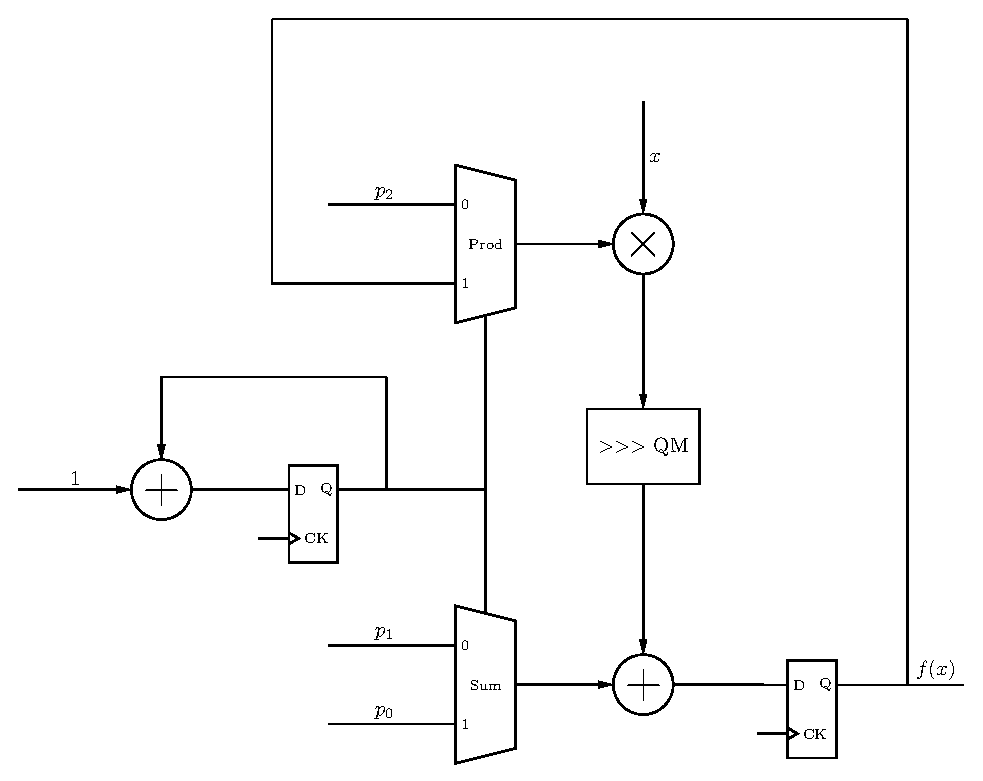
\includegraphics[width=0.9\linewidth]{figures/non-lin.eps}
    \caption[Block Diagram of the Non-linearity Calculator]{Block Diagram of the Non-linearity Calculator using a single multiplication. The multiplexer state is controlled by the flip-flip and sum block, that change state every clock cycle. When reset is applied, the selector is set to zero.}
    \label{fig:nonlin}
\end{figure}

\begin{figure}[H]
    \centering
    \begin{subfigure}{0.85\linewidth}
        \centering
        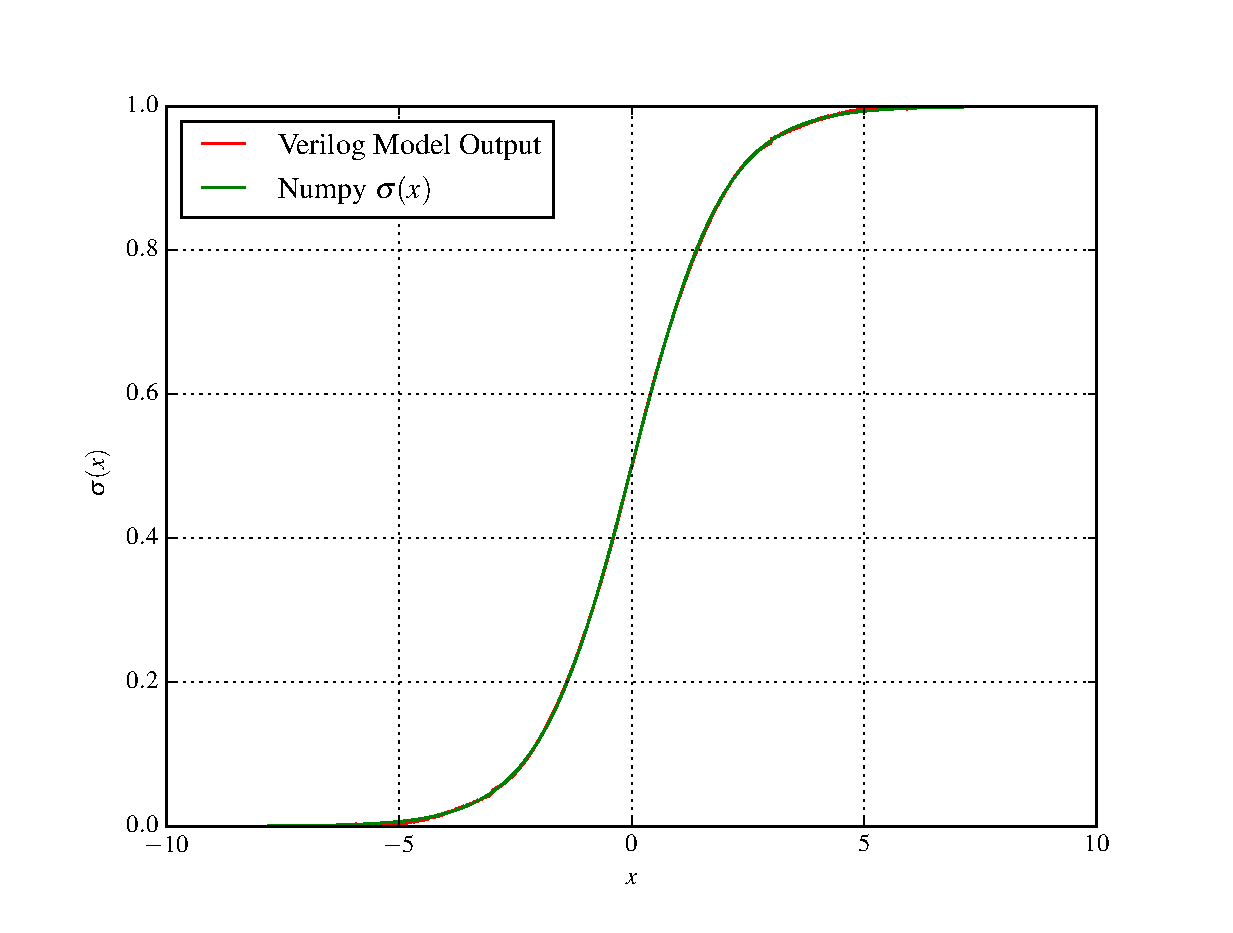
\includegraphics[width=\linewidth]{figures/nonlin-out.eps}
        \caption[Plot of the output of the Sigmoid Calculator HDL module]{Plot of the output of the Sigmoid Calculator HDL module}
        \label{fig:nonlin-out-sig}
    \end{subfigure}
    \begin{subfigure}{0.85\linewidth}
        \centering
        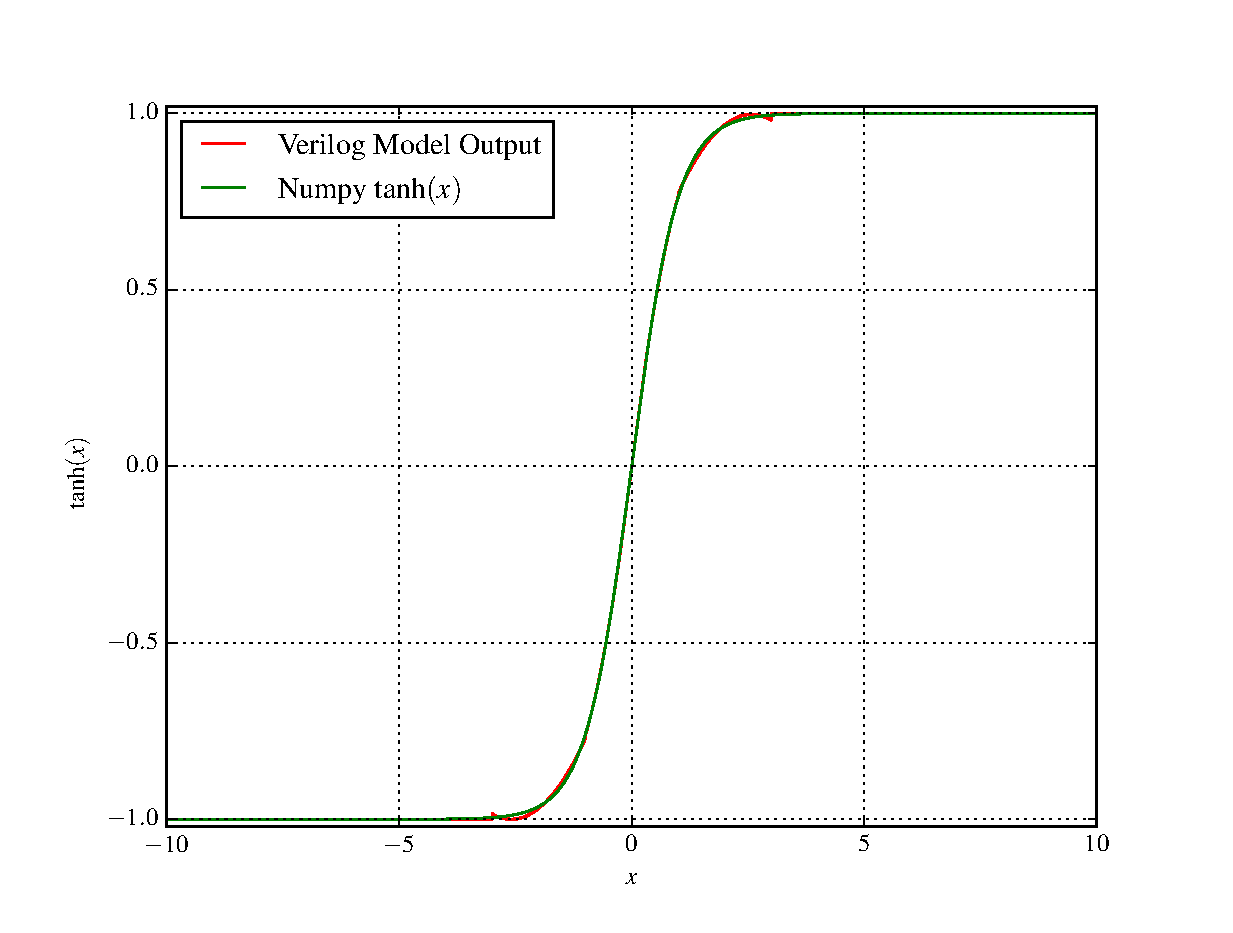
\includegraphics[width=\linewidth]{figures/nonlin-out-tanh.eps}
        \caption[Plot of the output of the Hyperbolic Tangent HDL module]{Plot of the output of the Hyperbolic Tangent HDL module}
        \label{fig:nonlin-out-tanh}
    \end{subfigure}
    \caption[The output of the HDL implementation of the activation functions]{The output of the HDL implementation of the activation functions}
    \label{fig:nonlin-out}
\end{figure}

\subsection{Matrix-vector Dot Product Unit}\label{sec:dotprod_sec}
From the set of Equations~\ref{eq:equationsLSTM}, we see that the weight matrices $\mb{W}_*$ and $\mb{R}_*$ are multiplied by the input vector $\mb{x}$ and the layer output vector $\mb{y}$, respectively. This way, we need a HDL block that implements matrix-vector multiplication, and that block must be parameterized in order to accomodate different matrices/vectors of various sizes: note that $x$ has length $M$ (the number of inputs to the layer), and so $\mb{W}_*$ has size $N\times M$, while $y$ has lenght $N$ (the number of neurons in the layer), and so $\mb{R}_*$ now has size $N\times N$. Plus, if we need a layer with different parameters, either in terms of number of inputs or number of neurons, it advisable to only change the respective parameter at the synthesis stage instead of having to redesign the whole block for that particular size. 

The matrix-vector dot product of a matrix $A$ of size $N \times M$ by a vector $x$ of size $M$, if performed in a linear non-parallel way, can be described in terms of Algorithm~\ref{matvec-alg}

\begin{algorithm}
\begin{algorithmic}
\For {$i$ = $1:N$}
    \For {$j$ = $1:M$}
    \State $y_i := y_i + A_{ij} \cdot x_j$
    \EndFor
\EndFor
\end{algorithmic}
\caption{Matrix-vector multiplication of a matrix}
\label{matvec-alg}
\end{algorithm}
This operation has a computational complexity of $O(n^2)$. It can be seen that each of the $i$-th component of the output vector $y$ can be calculated \textbf{in parallel}, each only requiring the corresponding $i$-th line from the matrix. If we follow this approach, matrix-vector multiplication can now be performed in \textbf{linear time}, which is one of the great advantages of custom-tailored hardware solutions. 

Although this solution only requires one multiplication per row of the input matrix (i.e. $N$ multiplications), if the row size is large, we may run out of resources in the FPGA; therefore, some sort of \textit{resource multiplexing} strategy must be used to ensure the flexibility of the solution to accomodate networks of larger dimensions. The solution I have found for this issue was to \emph{share} the multiplication slice between rows of the matrix: before, each multiplication slice was responsible for producing the $i$-th element of the output vector $y$ (of size $N$), therefore the final result for the vector would be ready in $M$ clock cycles (i.e. the number of columns); now, if we define a parameter $K_G = \frac{\text{Number of rows}}{\text{Number of multipliers}}$ -- the number of rows that share the same multiplier -- the same multiplier is responsible for producing several $i$-th elements of the output vector, in consecutive time slots of $M$ clock cycles. Suppose that we have a $8\times2$ matrix, and that $K_G = 2$; this way, we would have 4 multipliers, and the output vector elements $y_0$, $y_2$, $y_4$ and $y_6$ would be ready after $M=2$ clock cycles, and the remaining -- $y_1$, $y_3$, $y_5$ and $y_7$ --  are ready after another two clock cycles, that is $2M = 4$ clock cycles after the calculations began. 

In Figures-\ref{fig:mem-arrayprod} and~\ref{fig:array-prod} are depicted a diagram of the memory access for the Matrix, and the row multiplication and units within the module, respectively, where I have set $K_G = 4$, for the same matrix and vector sizes as before. Note that in this situation, we would only have 2 multipliers, and the module would be composed of two multiplication units, such as those in Figure~\ref{fig:array-prod}, that work in parallel: they address a particular column using the signal \verb+colSel+, which is used by the RAM module to output the corresponding column of the matrix (in regard to the input vector, obviously this signal selects only a single position), depicted in Figure~\ref{fig:mem-arrayprod}. The dark shaded part of the memory is used by the first multiplier, and the light shaded is used by the other, in parallel for a fixed \verb+rowMux+ -- this signal is produced by the control unit of the module, and essentially operates the left Mux and right Demux of Figure~\ref{fig:array-prod} that allows to choose the proper position of the weight column and to write to the correct output register, respectively. In this example, for \verb+rowMux+=0, the control unit increments \verb+colSel+ from 0 to $M$, and thus evaluating $y_0$ and $y_4$. After this, \verb+rowMux+ is incremented to 1, and the process repeats until \verb+rowMux+ reaches $K_G-1$. 

\begin{figure}
    \centering
    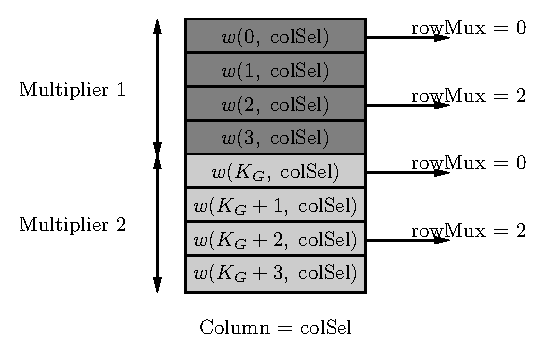
\includegraphics[width=0.9\linewidth]{figures/mem-array-prod.eps}
    \caption[A column of the matrix that serves as input to the module]{A column of the matrix that serves as input to the module. The dark shaded part is for the first multiplier, and the light shaded is for the other, in parallel. The rowMux signal addresses the position within each shaded area}.
    \label{fig:mem-arrayprod}
\end{figure}

\begin{figure}
    \centering
    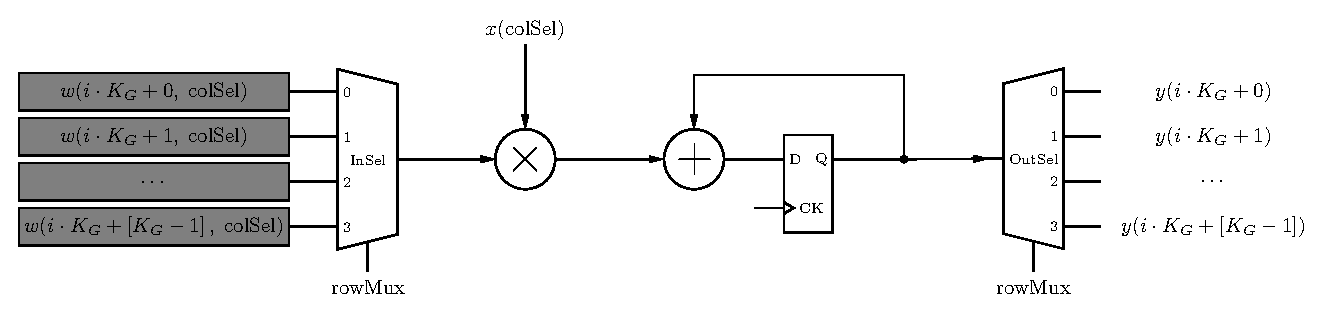
\includegraphics[width=\linewidth]{figures/array-prod.eps}
    \caption[The $i$-th row multiplication unit of the Module]{The $i$-th row multiplication unit of the Module, where rowMux and colSel are internal signals produced by the control unit of the module. The flip-flop accumulates the sum, and the output demux selects the appropriate memory position on where to store this value, within the slot attributed to this multiplication, from $i\cdot K_G$ to $i\cdot K_G + \left[K_G-1\right]$}
    \label{fig:array-prod}
\end{figure}
In summary, for an $N \times M$ weight matrix, this module outputs the result vector in $K_G \cdot M$ clock cycles.


\subsection{Dual-port Block RAM}
Although the bias weights, being simply a vector, I have chosen to keep them in normal registers and let the synthesis tool decide how to place them in the FPGA, for the weight matrices, the case is different. Since the
network size can be big, it is good to make sure that they are placed in the Block RAMs available in the FPGA. In Section~\ref{sec:dotprod_sec}, we see that, because of the architecture of the matrix-vector multiplier, it is convenient to have a column by column access to the weight matrix, and therefore this block outputs a given column in the \verb+rowOut+ output port terminal, at the \emph{negative edge} of the clock, selected by the value present in the input \verb+addressOut+ at the immediately previous \emph{positive edge} of the clock. As far as \textbf{writing} to the memory is concerned, the process is identical but now the column of weights at the input \verb+rowIn+ is sampled at \emph{negative edge} of the clock, and is placed at the column specified by the input \verb+addressIn+ at the previous \emph{positive edge} of the clock. 

Note that, for an $N \times M$ matrix, since the memory outputs and writes one column at a time, both the input and output port terminals will carry $N$ weights, and a total bitwidth of $\verb+BITWIDTH+ \cdot N$. 

The Verilog coding followed the Verilog Coding Guidelines in Xilinx's \href{http://www.xilinx.com/support/documentation/sw_manuals/xilinx2015_2/ug901-vivado-synthesis.pdf}{UG901} that, in page 50, recommends that the \verb+RAM_STYLE+ parameter be set to \verb+block+. This can be done by adding the follwing compiler directive before the register definition, as follows

\begin{verbatim}
(* ram_style = "block" *) reg [PORT_BITWIDTH-1:0] RAM_matrix [NCOL-1:0];
\end{verbatim}
where we can see that each register contains the respective column of the matrix, with $\verb+PORT_BITWIDTH+ = \verb+BITWDITH+ \cdot M$ and $\verb+NCOL+ = M$.
 

\subsection{Gate Module}

\subsection{Timing Diagrams of Operation}

\chapter{Results}\label{chap:results}
The optimized design of Section~\ref{sec:struct-shared} was synthesized for different network parameters, using Xilinx's Vivado 2015.4 Design Suite, and the synthesis results are reported in Section~\ref{sec:res-synth}, along with their discussion. The performance of the synthesized networks is very promising, showing an approximate $195\times$ speed-up over the LSTM Python model, which was running on a high-end desktop computer with an over clocked CPU. Although the FPGA aims for an Embedded System environment usage, the fairness of this comparison still holds, since a Python/Numpy implementation is slower than a lower-level language implementation (such as in C) and this level of performance would be similar to a C implementation in a low-power, embedded CPU platform. These results are reported in Section~\ref{sec:res-valid}. 

\section{Synthesis}\label{sec:res-synth}
In order to assess the impact of the network size on the performance and resource usage of the proposed design, I have synthesized the Verilog description of the proposed network for sizes $N$ of 4, 8, 16 and 32, and for each of these the resource sharing parameter $K_G$ was also varied (as will be explained further ahead, the number of inputs is set to $M=2$). Since performance is the key factor for using an FPGA implementation, the synthesis strategy used was the \verb+Flow_PerfOptimized_high+, and the implementation strategy was \verb+Performance_ExplorePostRoutePhysOpt+ to perform a post-route optimization stage that proved useful in many cases to meet the clock specifications when the first Place\&Route pass failed to meet them. For a network size of 32 and $K_G=8$, the LUT usage exceeded the LUT resources available in the FPGA, so only lower values of $K_G$ were successfully synthesized.
 
\subsection{Maximum Frequency}\label{sec:res-synth-maxfreq}
Using the synthesis strategy outlined in the previous paragraph, the maximum clock frequency that does not cause timing violations of any sort is plotted in Figure~\ref{fig:maxfreq}. For $N=4$, since there are only 4 rows to be multiplied, the maximum value of $K_G$ is 4, and hence no synthesis was performed for $K_G = 8$; also, since $K_G = 2$ and $N=32$ would use $32(8/2+3) = 224$ DSP slices, that exceeds the 220 slices available in the Zynq 7020, so there is no synthesis data for that value.

First, for all network sizes, it is clear that with increasing $K_G$, the maximum clock speed decreases. This means that there is a critical path in the Matrix-Vector multiplication unit, whose multiplexer becomes increasingly complex for higher values of $K_G$. On the other hand, when $K_G$ is the same, smaller networks are faster than larger networks. The fastest design is an $N=4$ and $K_G = 2$ network, with a clock frequency of $140.154$ MHz, and the slowest one is an $N=32$ and $K_G=4$ network, clocked at $90.498$ MHz. The reference design used for validation in Section~\ref{sec:res-valid} is an $N=8$ and $K_G=2$ network is clocked at $132.89$ MHz, which yields a clock period of $7.525$ ns.

\begin{figure}
    \centering
    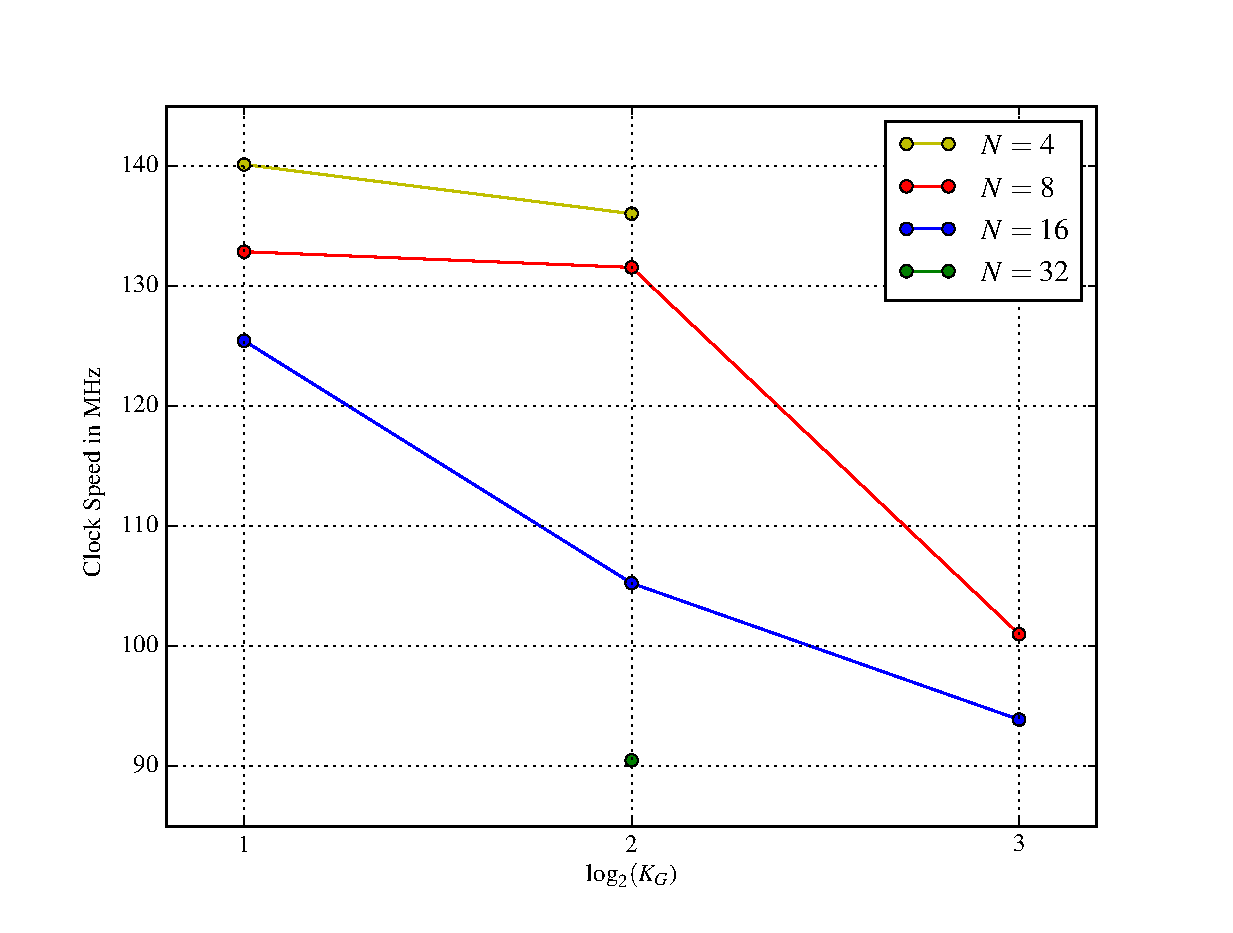
\includegraphics[width=\linewidth]{figures/maxfreq.eps}
    \caption[The maximum achievable clock frequency for several Network Sizes $N$ and resource sharing level $K_G$]{The maximum achievable clock frequency for several Network Sizes $N$ and resource sharing level $K_G$}
    \label{fig:maxfreq}
\end{figure}


\subsection{DSP Slices Usage}\label{sec:res-synth-dsp}
The estimates made in Equation~\ref{eq:numdsp_network-opt} were proven to be accurate, as Figure~\ref{fig:dspused} confirms. The reference network design uses 56 DSP slices, which corresponds to $25.45\%$ of the total number of DSP slices available.
\begin{figure}
    \centering
    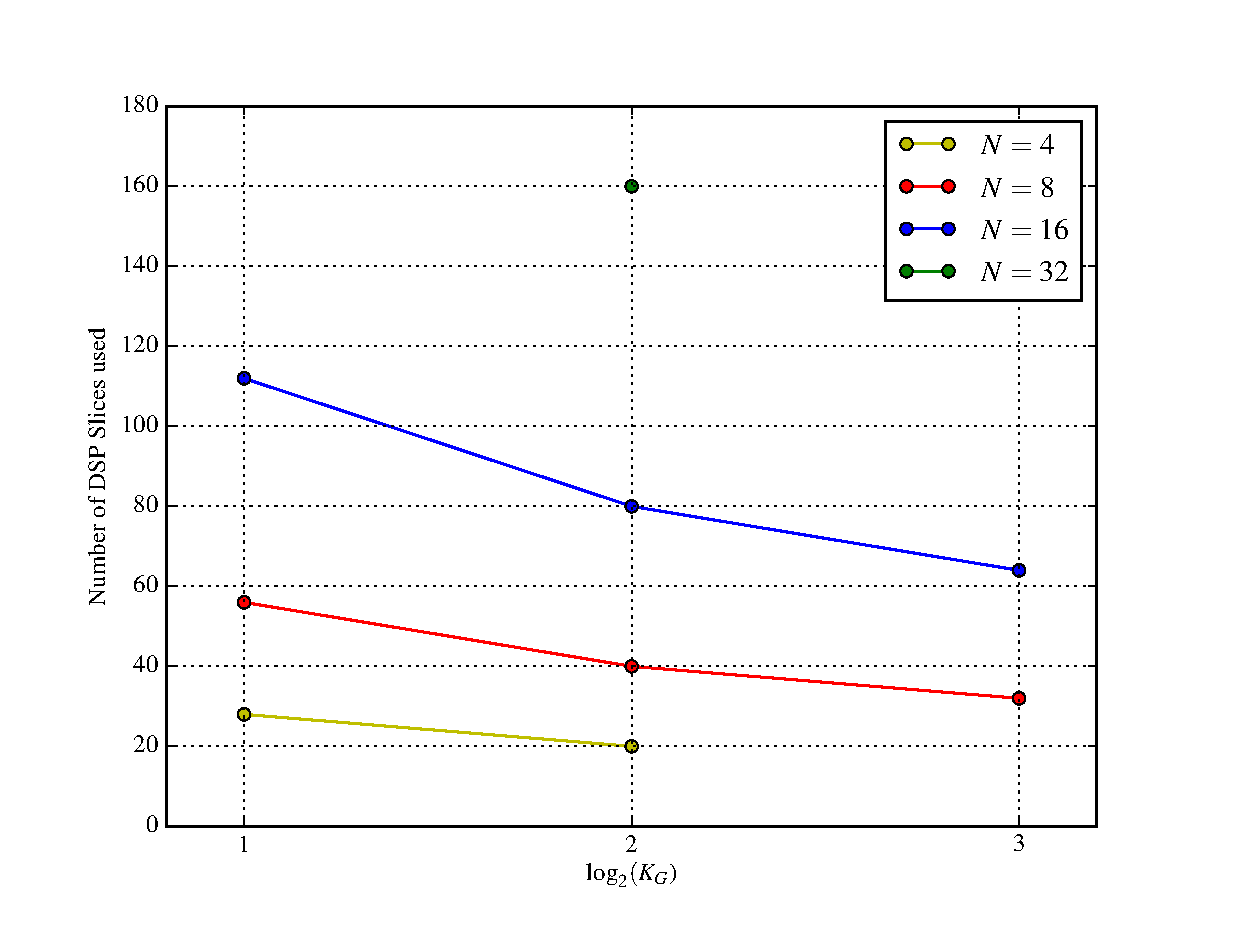
\includegraphics[width=\linewidth]{figures/dspuse.eps}
    \caption[The number of DSP slices used for several Network Sizes $N$ and resource sharing level $K_G$]{The number of DSP slices used for several Network Sizes $N$ and resource sharing level $K_G$}
    \label{fig:dspused}
\end{figure}

\subsection{Power Usage}\label{sec:res-synth-power}
Another important metric of the performance of a design is its \textbf{power consumption}. All designs yielded a constant baseline value for the \emph{static} power consumption of around 120 mW, and the power consumption reported in Figure~\ref{fig:power} refers to the \emph{total} power consumptions, i.e. both the baseline static power and the dynamic power consumption. It is clear that the smaller the network is, the less power is consumed, as one would expect. Furthermore, an increasing level of resource sharing yields a substantially lower power consumption figure: this is because we use less DSP slices when we increase $K_G$. Of course, even though the power consumption is lower in that case, that comes at the expense of a lower clock frequency and more clock cycles elapsed per forward propagation.

\begin{figure}
    \centering
    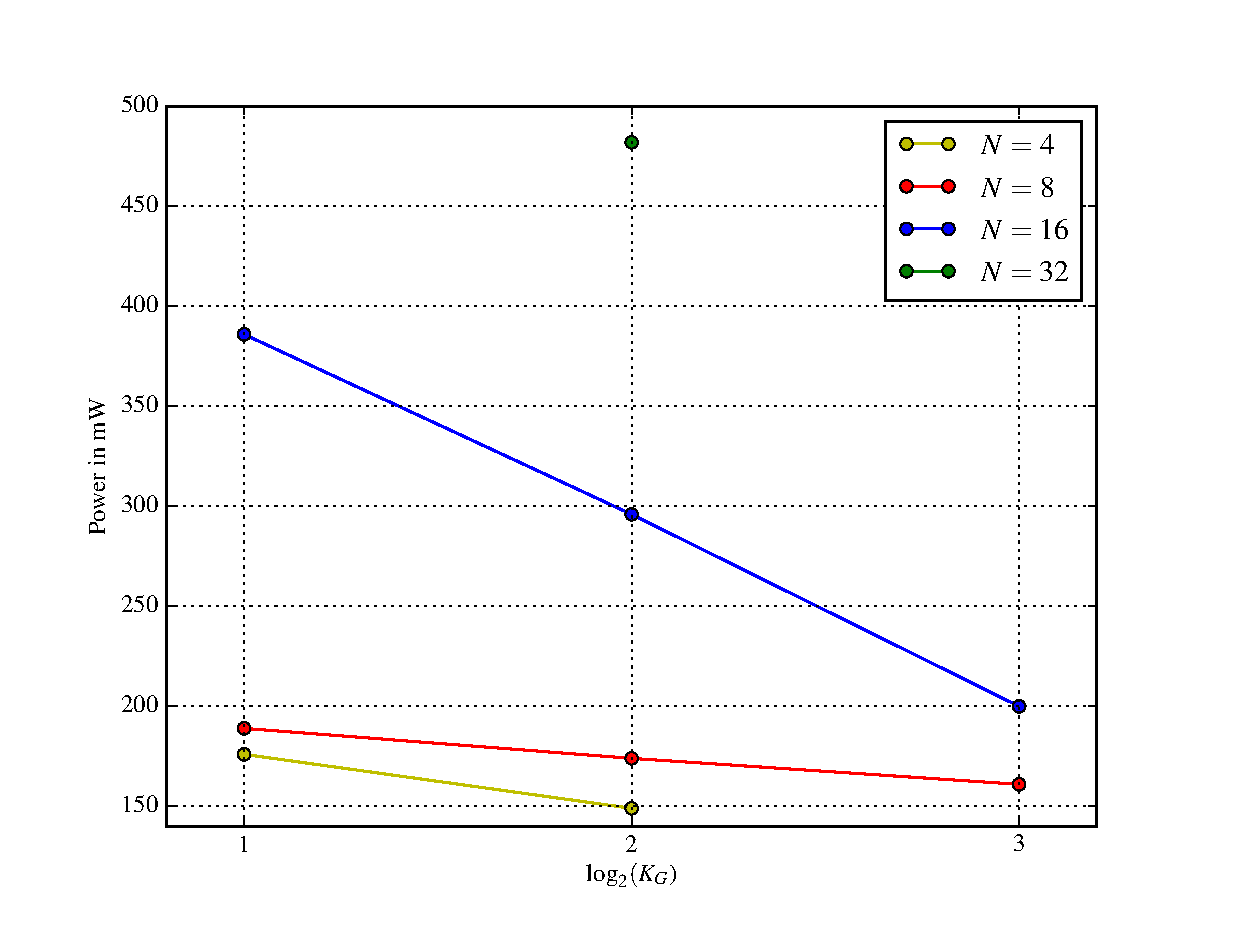
\includegraphics[width=\linewidth]{figures/power.eps}
    \caption[Power consumption estimates for several Network Sizes $N$ and resource sharing level $K_G$]{Power Consumption estimates for several Network Sizes $N$ and resource sharing level $K_G$}
    \label{fig:power}
\end{figure}

\subsection{Other Resources Usage}\label{sec:res-synth-otheres}
Besides DSP slices, it is also worth mentioning the usage of LUT, LUTRAMs and Flip-Flops. In Table~\ref{tab:lut}, the usage of LUTs is reported, where we can see that although there is not a clear trend on how the LUT usage varies with increasing $K_G$, it is clear, and expectable, that the LUT usage increases with the size of the network by an approximate factor of 2, from $N=2$ to $N=16$. As for $N=32$, the usage does not follow this apparent trend, and rises sharply to 91\%. For $K_G = 8$ the usage even surpasses the maximum amount of LUTs available.
\begin{table}
    \centering
  \begin{tabular}{ | l | c | c | c |}
    \hline
    & $K_G=2$  & $K_G=4$ & $K_G=8$ \\ 
    \hline
    $N=4$ & 6.87\% & 6.04\% & N.A. \\    
    \hline
    $N=8$ & 14.64\% & 13.03\% & 14.11\% \\    
    \hline
    $N=16$ & 28.97\% & 27.72\% & 29.85\% \\    
    \hline
    $N=32$ & N.A. & 91.09\% & N.D. \\    
\hline
  \end{tabular}
    \caption{LUT usage for different $N$ and $K_G$}
    \label{tab:lut}
\end{table}

As for LUT, the FF usage also scales accordingly to a $2\times$ factor. Furthermore the LUTRAM usage scales well and does not pose a limitation on the network size. The usage results are reported in Table~\ref{tab:ff}.

\begin{table}
    \centering
  \begin{tabular}{ | l | c | c |}
    \hline
         & LUTRAM  & FF  \\ 
    \hline
    $N=4$ & 0.18\%  & 3.39\% \\    
    \hline
    $N=8$ & 4.41\%  & 6.7\% \\    
    \hline
    $N=16$ & 8.83\%  & 13.36\% \\    
    \hline
    $N=32$ & 17.66\% &  26.45\% \\    
\hline
  \end{tabular}
    \caption{Flip-flop usage for different $N$ and $K_G$}
    \label{tab:ff}
\end{table}

\section{Validation and Comparison}\label{sec:res-valid}
Over the course of this Section, the functionality of the network is verified against the Python reference module of~\ref{sec:res-pyth} that I have developed as a reference, both for the forward propagation of the network, as well as for the training algorithm. The methodology of this procedure is outlined in Section~\ref{sec:res-meth}. On Section~\ref{sec:res-valid-fpps}, I will assess how the performance results of Section~\ref{sec:res-synth-maxfreq} translate into how many classifications per second this design achieves, and how that figure compares with the capabilities of the Python module.

\subsection{Reference Python Module}\label{sec:res-pyth}
Before performing the Verilog description of the network, I have tested the ideas outlined in Section~\ref{chap:theorBack} first by building a software version of an LSTM Network. Since I wanted to quickly test the ideas without much effort, I decided to use Python and Numpy rather than MATLAB, since the former have higher performance at the same level of code complexity. The code for this Python class is listed in Appendix~\ref{ap1:lstm-pyth}. It supports both the forward propagation of an already trained network, but also provides functions to train a model using the SPSA method outlined in Section~\ref{sec:training_lstm} and also Backpropagation Through-Time as presented in~\cite{Greff15}. As the reader can attest by running the code himself, the SPSA proves to be a valid approach for training these networks, achieving convergence for the Machine Learning task that will be presented in the next paragraph, although it converges slower than Backpropagation Through Time.  

The learning problem presented to both the software and hardware network is the sum of two binary numbers of 8 bits. The bits of each number at position $i$ are input to the network as a vector, and the network outputs its prediction of the correct value of the $i$-th bit of the \emph{result} number. After the whole number number is processed, the memory cells of the LSTM network are reset and a new addition task can be presented to the network. Even though this seems a rather simple problem, it accounts for all the essential issues at which this network excels: first, this is a \emph{classification} problem in which the Machine Learning algorithm needs to output a prediction based on the input feature vector, and that prediction has to take into account the \emph{history} of predictions so far, because the current bit is the sum of not only the bits of the two operands, but also the \emph{carry} generated at the last few positions -- this is where the memory cells of this special Neural Network come into effect.  

\subsection{Methodology}\label{sec:res-meth}
The Python testbench that both trains and verifies the predictions of the software network of Appendix~\ref{ap1:lstm-pyth} is listed in Appendix~\ref{ap1:testbench-pyth}. This script, after achieving convergence, stores the trained network weights in \href{https://docs.python.org/3/library/pickle.html}{Pickle} format. These weights are, then, converted to $Q6.11$ fixed-point format and directly loaded into the Verilog model by the Verilog testbench. The Verilog testbench then applies in order the bits of randomly generated numbers, captures the output bit and checks whether it is correct or not, and counts the number of incorrect bits.

This network has, then, two inputs ($M=2$) and eight neurons ($N=8$). Furthermore, the output of the eight LSTM neurons is reduced to a single output by means of a simple neuron, as the one described in Figure~\ref{fig:modelNeuron_a}. This introduces a further 5 clock cycle overhead that is not accounted in Section~\ref{sec:res-valid-fpps}, since it is not actually part of the LSTM Network and, although it was placed in series in the datapath, after the LSTM network, it can run in parallel with the LSTM network, introducing no overhead whatsoever.

A Python script was written (see Appendix~\ref{ap1:runtb-lstm}) to automatically compile the Verilog code, generate the input and output data, and call Questasim to run the simulation of the HDL code. Figure~\ref{fig:res-meth-wave} shows the waveform viewer window of a run of the Verilog testbench, and in Appendix~\ref{ap1:transcript-cmd} shows the transcript of a successful run of this testbench, proving that the learning ability of the Hardware network still retains the predicting capability of the software network. 

\begin{figure}
    \centering
    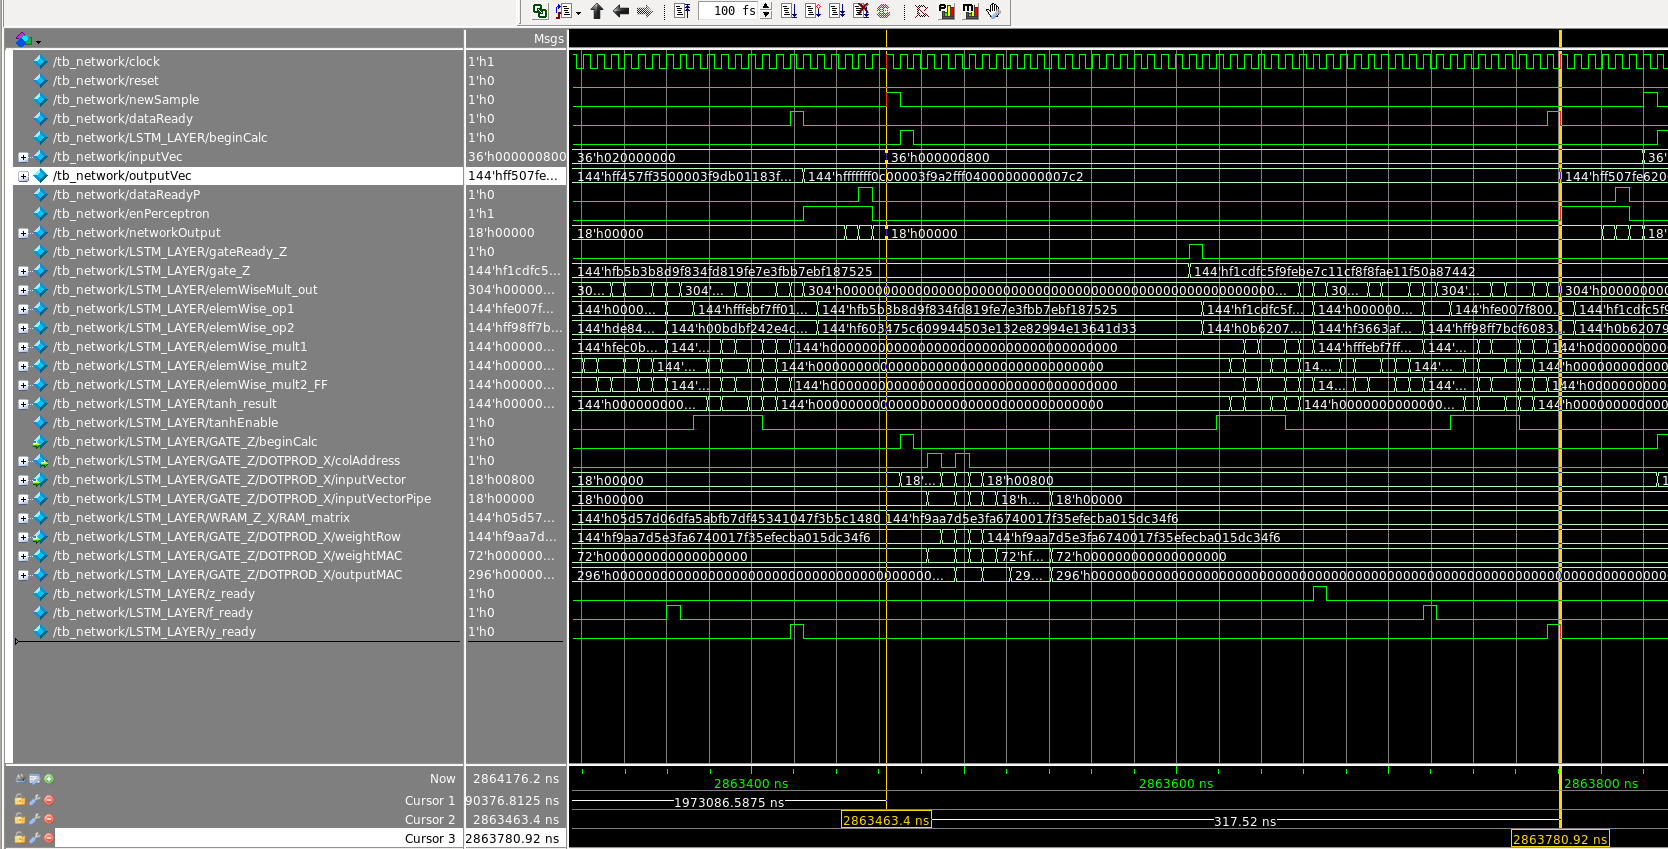
\includegraphics[width=\linewidth]{figures/wave.png}
    \caption[Screenshot of the simulation run of a complete forward propagation for $N=8$ and $K_G=2$]{Screenshot of the simulation run of a complete forward propagation for $N=8$ and $K_G=2$. The period between the two time cursors is the same as the one reported in Table~\ref{tab:process-time}}
    \label{fig:res-meth-wave}
\end{figure}
\subsection{Performance}\label{sec:res-valid-fpps}
To evaluate the performance of the network in terms of how fast it can produce data, I have defined a metric based on how many predictions it can produce per second (i.e. produce a new result bit in the output sequence), in \textbf{millions}. The prediction time is the time elapsed since a new input vector is applied \emph{to} the moment the LSTM Network produces an output vector (as discussed previously, the five clock cycles of the simple neuron at the output are \textbf{not} considered). To do this, we multiply the number of clock cycles yielded by Equation~\ref{eq:numcc_network-opt} by the equivalent clock period from the synthesis clock report of Figure~\ref{fig:maxfreq}. This result is epitomized in Table~\ref{tab:process-time}, where the calculation time of the Python module forward propagation function is also included. This time was measured using the \href{https://docs.python.org/3.5/library/timeit.html}{\textbf{timeit}} module, that allows the evaluation of the execution time of small pieces of code as well as complete functions with arguments. The Python code was run on a Linux System, powered by an i7-3770k Intel Processor, running at 4.2GHz.

\begin{table}
    \centering
    \begin{tabular}{ | l | c | c | c | c | c | }
    \hline
    & $K_G=8$  & $K_G=4$ & $K_G=2$ & Python & Speed-up \\ 
    \hline
    $N=4$ & N.A.  & 360.15 ns  & 292.535 ns & 65 $\mu$s & $\times180$ \\   
    \hline 
    $N=8$ & 960.3 ns  & 494 ns  &  368.725 ns & 72 $\mu$s & $\times194$ \\    
    \hline
    $N=16$ & 1.715 $\mu$s  & 921.5 ns  & 518.05 ns & 96 $\mu$s & $\times185$ \\
    \hline
    $N=32$ & N.D. & 1.78 $\mu$s  & N.A. & 185 $\mu$s  &  $\times104$ \\    
\hline
  \end{tabular}
    \caption{Total processing time for a single forward propagation, for hardware networks of various $K_G$ and the Python software network of equivalent size. The speed-up figure is calculated between the Python processing time versus the best hardware network time of the same size}
    \label{tab:process-time}
\end{table}
The performance increase is impressive, even for the slowest of the designs (the $N=32$ network). The hardware network is, at best, $\times200$ faster than the software counterpart, and at worst $\times100$ faster. Also, it is noticeable that increasing the level of resource sharing increases the computation time, since the level of parallelism is lower. 

 Since the previous values are the time needed for a \emph{single} forward propagation, to know how many forward propagations we can perform \emph{per second}, we only need to invert the previous values. These values are presented in Figure~\ref{fig:Mclass-psec}. While the $N=8$ and $K_G=2$ network is able to perform around 3.2 million predictions per second, the Python model can only output around 14 thousand predictions, which is a very significant result that proves the relevance of this implementation.
\begin{figure}
    \centering
    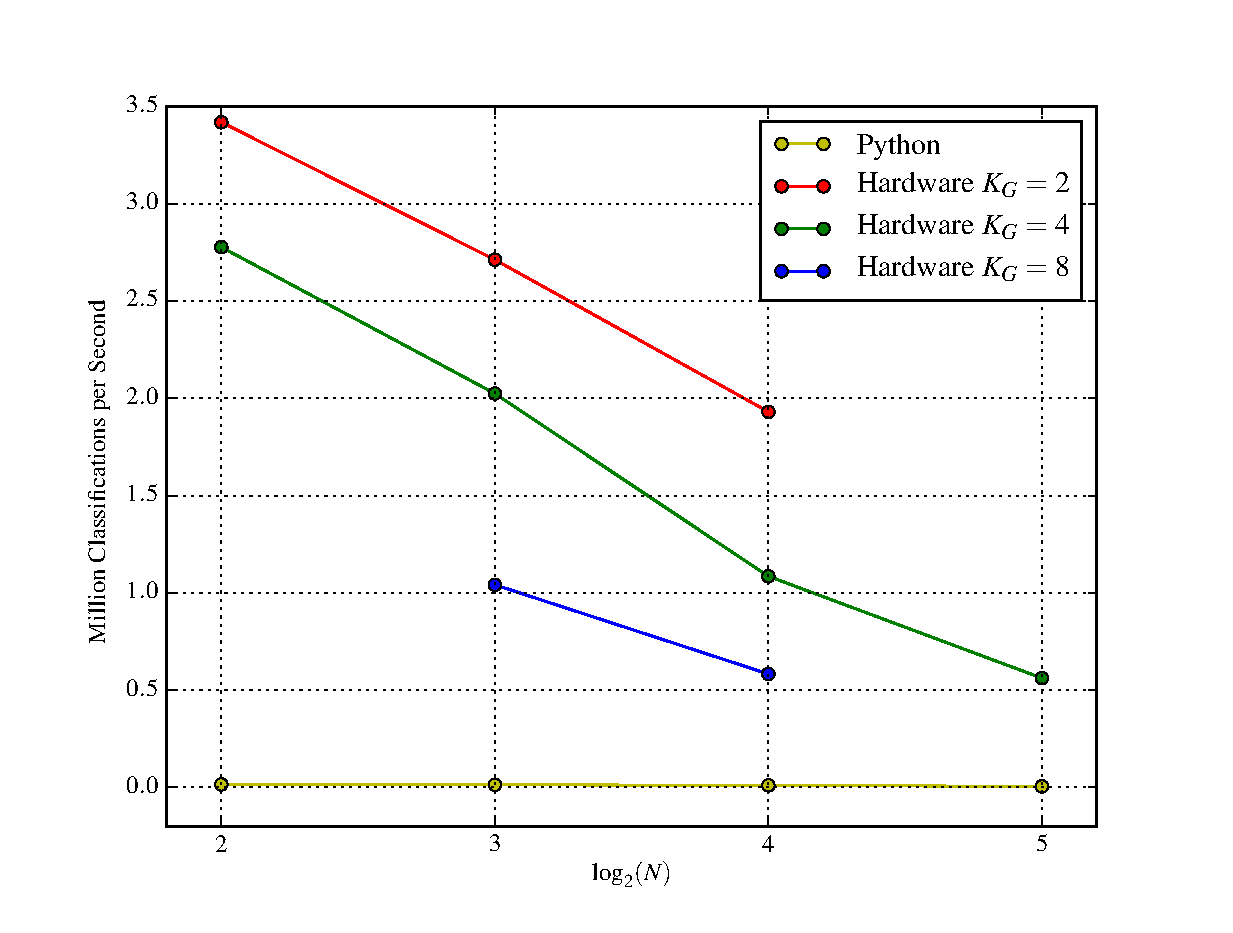
\includegraphics[width=\linewidth]{figures/Mclass-psec.eps}
    \caption[Millions of classifications per second of each design according to the network size $N$]{Millions of classifications per second of each design according to the network size $N$. The comparison is between the software Python model and 3 networks of different levels of resource sharing $K_G$.}
    \label{fig:Mclass-psec}
\end{figure}





%% comment next 2 commands if numbered appendices are not used
%\appendix
%\chapter{Loren Ipsum} \label{ap1:loren}

Depois das conclusões e antes das referências bibliográficas,
apresenta-se neste anexo numerado o texto usado para preencher a
dissertação.

\section{O que é o \emph{Loren Ipsum}?}


\section{De onde Vem o Loren?}


%%----------------------------------------
%% Final materials
%%----------------------------------------

%% Bibliography
%% Comment the next command if BibTeX file not used
%% bibliography is in ``myrefs.bib''
\PrintBib{bibliography}
%\bibliographystyle{IEEETran}
%\bibliography{bibliography}
%% Index
%% Uncomment next command if index is required
%% don't forget to run ``makeindex thesis'' command
%\PrintIndex

\end{document}
